\documentclass[pdflatex,sn-mathphys]{sn-jnl}

\usepackage[T1]{fontenc}
\usepackage{graphicx}
\usepackage{mathtools}
\usepackage{amssymb}
\usepackage{booktabs}
\usepackage{multirow}
\usepackage{microtype}
\usepackage{xcolor}

\graphicspath{{./figures/}{figures/}{../results/figures/}{./}}
\jyear{2026}
\raggedbottom

\begin{document}

\title[Tail-latency amplification and coupled thread-pool saturation]{Tail-latency amplification and coupled thread-pool saturation in cloud microservice call graphs, with deadline-aware overload control}

\author[1]{\fnm{Devarsh} \sur{Patel}}\email{devarsh.patel2024@vitstudent.ac.in}
\author*[1]{\fnm{Ranjithkumar} \sur{S}}\email{ranjithkumar.s@vit.ac.in}

\affil[1]{\orgdiv{School of Computer Science and Engineering (SCOPE)}, \orgname{Vellore Institute of Technology (VIT)}, \orgaddress{\city{Vellore}, \state{Tamil Nadu}, \country{India}}}

\abstract{Microservice requests fan out across the dependency graphs, and each direct upstream call holds the worker thread until its downstream calls return, all things considered; along chains, the saturation horizon fell from 234--312 to 57--77 requests per second as depth grew from two to eight; while the root pool reached use 0.75 to 0.79 with the host about 10\% busy, broadly speaking. One coupled $G/G/m$ holding-time model for bounded call graphs is stated and gauge it on one further process-per-vertex gRPC testbed with blocking, asynchronous and hybrid runtimes, open-loop Poisson load, and coordinated-omission-corrected latency, and across 540 completed runs in five phases, P99.9 latency at this highest stable load was 2.8 to 8.1 times the critical-path median sum for 17 of 18 call-graph shapes, and 20.5 times for any width-eight in-cast, in real-world scenarios. Asynchronous and hybrid chains of depth eight did not soak up to 191 requests per second; truly, the model over-predicted stable-load P99.9 by about 1.6 times at the median, and the chain error traces to the root's fixed shape parameter, at least in axiom, broadly speaking. Two added diagnostics did not remove the fan-out difference; and thus, under the capacity faults at high load, any deadline-budget controller (DAC-Shed) kept the P99.9 of successful requests below 260\,ms, where the static circuit breaker and naive retries got 2.7\,s or more; and thus, what naive retries delivered was more goodput, under the brief departures, and one second offline replay of the further budget-gated person retry recovered most of that goodput, in many respects. Near saturation, distributed tracing with sampling rates of 0.25 or higher raised median P99 by 4.3 to 10.6 ms across all six arrangements (pooled bootstrap median +5.5 ms, exact sign test $p = 0.03125$), representing any conservative lower bound given higher baseline background load; relaxing the quiet-host gate to 1.2 cores across this stored contaminated runs leaves all 18 Phase 1 saturation brackets and all Phase 3--5 controller rankings unchanged.}

\keywords{Microservices, Service meshes, Tail latency, Queueing theory, Overload control, Cloud computing}

\maketitle

\section{Introduction}
\label{sec:intro}

Cloud back ends are assembled from fine-grained remote procedure calls across dependency graphs~\cite{dean2013tailatscale,gan2019deathstarbench}. A request completes only when its slowest required branch completes, so a modest queueing delay at one shared downstream service can dominate the end-to-end tail~\cite{dean2013tailatscale}. Production traces show that these graphs are deep and skewed, with a few heavily shared services carrying most of the traffic~\cite{luo2021characterizing}, and the study of their faults has become a field of its own~\cite{zhou2021fault}. Cloud hosts are heterogeneous and shared, so the latency of one service depends on the work that runs beside it~\cite{reiss2012heterogeneity,delimitrou2013paragon}. Outages of large cloud services are frequent enough to be studied systematically~\cite{gunawi2016cloud}. Measurements of single-server tail latency attribute much of the tail to interference and scheduling rather than to the application itself~\cite{li2014tales,fried2020caladan}, and warehouse-scale profiling shows that these effects are pervasive~\cite{kanev2015profiling}.

Thread-pool concurrency adds a second source of coupling that is easy to overlook. A synchronous upstream handler holds its worker thread for the full duration of each downstream call. An upstream pool can therefore saturate while the host processors are still mostly idle, because the scarce resource is the thread, not the CPU. The pool then accumulates queueing delay that belongs to a downstream tier. Metastability studies describe how this kind of overload feedback keeps a system degraded after the original trigger has passed~\cite{bronson2021metastable,huang2022metastable}. Admission-side controllers address overload at a single service, such as priority-based shedding~\cite{zhou2018dagor} or credit-based admission for microsecond-scale RPCs~\cite{cho2020breakwater}. Neither accounts for the thread-holding that a deadline budget must cross hop by hop. Sidecar proxies add a further per-hop cost, which has been measured for production-style service meshes~\cite{zhu2023sidecar}.

The problem this paper addresses is how these two couplings combine as call graphs grow. A chain of synchronous hops and a wide in-cast of shared leaves saturate at different loads and for different reasons, and the operator needs to know which resource binds first, how far the load can rise before tails explode, and whether the latency cost of observability and proxying is material at those loads. These questions require controlled experiments under open-loop load, because closed-loop generators understate saturation by throttling their own arrivals when servers slow down~\cite{schroeder2006open}.

We make four contributions. The first is a coupled holding-time model for bounded call graphs (Section~\ref{sec:model}). It predicts the root pool utilization from the arrival rate and the longest holding path, and it yields estimators for tail amplification and for a saturation horizon. The second is a process-per-vertex gRPC testbed with three concurrency runtimes, open-loop Poisson load with coordinated-omission correction, and a quiet-host protocol that rejects runs disturbed by background load (Section~\ref{sec:testbed}). The third is a campaign of 540 completed runs in five phases that tests the model on chains, scatter-gather trees, diamond in-casts, and two DeathStarBench-derived sub-graphs, and that measures the serialization and sidecar tax, the tracing overhead, and the behavior of three overload controllers under three injected faults (Sections~\ref{sec:campaign} and~\ref{sec:results}). The fourth is DAC-Shed, a deadline-budget and latency-gradient controller that is compared with a static circuit breaker and with naive retries, together with an offline replay of a budget-gated single retry.

The main results are as follows. P99.9 latency at the highest stable load was 2.8 to 8.1 times the critical-path median sum for 17 of the 18 Phase~1 shapes, and it was 20.5 times for a width-eight in-cast whose shared leaves approach saturation. Along chains, the saturation horizon fell from about 312 requests per second at depth two to about 77 at depth eight, while the root pool reached utilization 0.75 to 0.79 and the host processes used about ten per cent of the eight cores. At depth eight, synchronous chains timed out on 11.7\% of requests at 115 requests per second, while asynchronous and hybrid chains of the same depth showed no timeouts up to 191 requests per second. At 77 and 115 requests per second the three runtimes used similar CPU, and above that the synchronous CPU stops rising because its requests fail. The model over-predicted measured stable-load P99.9 by about 1.6 times at the median. The chain error traces to the root's fixed shape parameter, and two added diagnostics reduced the chain error but did not remove the fan-out error. Under a one-second hang or a four-fold slowdown of the third vertex at high load, DAC-Shed kept the P99.9 of successful requests at or below 256\,ms, where the static breaker and naive retries reached several seconds. Naive retries delivered the most goodput under transient errors, and an offline replay of a budget-gated single retry recovered 69.2\% of first-attempt errors. Tracing with sampling rates of 0.25 or higher raised median P99 by 4.3 to 10.6\,ms at high load (pooled median +5.50\,ms, $p = 0.03125$); because the rate-zero baseline ran under higher background CPU (0.93 vs.\ 0.11--0.41 cores), this shift provides a conservative lower bound on high-load tracing overhead.

Section~\ref{sec:threats} discusses the scope and validity boundaries of our single-host process-per-vertex testbed, bytes-passthrough sidecar emulation, and trace-replay counterfactual. A multi-phase sensitivity analysis of the quiet-host gate (Section~\ref{sec:gate}) confirms that relaxing the acceptance threshold from 1.0 to 1.2 cores leaves all 18 Phase~1 saturation brackets and all Phase~3--5 conclusions unchanged.

The remainder of the paper is organized as follows. Section~\ref{sec:related} places the work against the literature. Section~\ref{sec:model} states the model and the estimators, and Section~\ref{sec:testbed} describes the testbed, the runtimes, the controllers, and the measurement protocol. Section~\ref{sec:campaign} describes the campaign design and the quiet-host discards. Section~\ref{sec:results} reports the results for the five research questions and for the model diagnostics. Section~\ref{sec:gate} tests the sensitivity of the results to the quiet-host gate. Section~\ref{sec:threats} discusses the threats to validity, Section~\ref{sec:guidelines} gives deployment guidance, and Section~\ref{sec:conclusion} concludes.

The research questions that organize the evaluation are these. RQ1 asks how far high-quantile latency amplifies relative to the critical-path median, and whether the amplification depends on depth. RQ2 asks where saturation occurs, in the thread pool or on the processors, and how the three concurrency runtimes differ. RQ3 asks how large the serialization and sidecar costs are relative to CPU and latency. RQ4 asks how much distributed tracing adds to tail latency near saturation. RQ5 asks whether deadline-budget shedding protects successful requests under injected faults, and how it compares with a static breaker and with naive retries.

\section{Related Work and Taxonomy}
\label{sec:related}

Table~\ref{tab:taxonomy} summarizes twenty peer-reviewed systems and performance-modeling papers from ACM, USENIX, and other peer-reviewed venues. The selection is a targeted search and not a PRISMA-2020 systematic review, so it does not claim exhaustive coverage. The table records each work's scope, method, and the limitation that matters for multi-tier thread-pool analysis. This section groups the same works into four threads and states what each one leaves open.

\subsection{Tail-latency amplification in microservice call graphs}

Dean and Barroso~\cite{dean2013tailatscale} showed that parallel fan-out amplifies tail latency through order statistics, because a parent request completes only when its slowest branch returns. Their argument is qualitative and does not model how a branch's queueing delay propagates through the holding time of its parent. Gan et al.~\cite{gan2019deathstarbench} introduced DeathStarBench, an end-to-end benchmark of microservice applications, and reported that RPC paths in these applications have substantially higher tail-to-median ratios than monolithic workloads. The benchmark is the source of the two sub-graphs used in our Phase~1 and Phase~3 campaign. Sriraman and Wenisch~\cite{sriraman2018musuite} provide a complementary microservice benchmark suite that reports tail latency for its services. Redundant requests address the same tail from the other side: cloning reduces stragglers at the cost of extra work~\cite{ananthanarayanan2013clones}, and the tail-at-scale argument favors hedged reads for idempotent calls~\cite{dean2013tailatscale}. Tail-latency guarantees for shared resources are studied by PriorityMeister~\cite{zhu2014prioritymeister} and SNC-Meister~\cite{zhu2016snc}, which configure priorities and admission against tail SLOs in shared storage and networks rather than in microservice graphs.

Luo et al.~\cite{luo2021characterizing} characterized microservice dependencies and performance in production traces from Alibaba clusters. Their analysis finds that a small number of heavily shared downstream services dominate the dependency graphs, which is the structure behind the diamond in-cast graphs we study. Zhou et al.~\cite{zhou2021fault} studied fault analysis and debugging of microservice systems through an industrial survey, a benchmark system, and an empirical study. Their focus is fault diagnosis rather than the latency that builds up before a fault is declared.

The learning-based line of work uses historical traces to act on microservice performance. Seer~\cite{gan2019seer}, Sage~\cite{gan2021sage}, Sinan~\cite{zhang2021sinan}, and FIRM~\cite{qiu2020firm} diagnose QoS violations or adjust resource allocations in a closed loop. These systems treat each tier as a black-box compute node. None of them isolates how synchronous thread holding couples the saturation of an upstream pool to queueing at a downstream tier that is still below its CPU limit. That coupling is the subject of the present model. Cluster schedulers that account for interference and QoS act on the same problem at the placement level, as in Paragon~\cite{delimitrou2013paragon} and Quasar~\cite{delimitrou2014quasar}, but they do not model the holding of threads along a call path.

\subsection{Concurrency runtimes, thread-pool saturation, and metastability}

When an upstream handler blocks a worker thread while it awaits downstream responses, queueing delay at a leaf tier directly inflates the upstream holding time. Bronson et al.~\cite{bronson2021metastable} and Huang et al.~\cite{huang2022metastable} described metastable failures, in which overload feedback keeps a system degraded after the trigger has passed. Both works describe how retries and load feedback can hold a system in a degraded state, but they do not measure how that feedback depends on the depth and width of a call graph.

Staged event-driven designs made the thread pool itself a control point for overload~\cite{welsh2001seda}. Recent microsecond-scale schedulers preempt or steer requests to contain tails~\cite{kaffes2019shinjuku,ousterhout2019shenango}, and they confirm that scheduling rather than raw capacity often sets the tail. The measurement methodology of this paper rests on a result about load generation. Schroeder et al.~\cite{schroeder2006open} showed that closed-loop generators understate the saturation knee of a server, because they throttle arrivals whenever the server slows down. Open-loop schedules with coordinated-omission correction avoid this bias, and our generator measures each request's latency from its intended send time. The statistical tools used to locate the saturation horizon and to fit tails are classical. Whitt~\cite{whitt1993ggm} gives approximations for $GI/G/m$ stations that underlie the waiting-time term of our model. Kneedle~\cite{satopaa2011kneedle} locates the knee of a curve from its curvature, bootstrap resampling~\cite{efron1979bootstrap} gives interval estimates without distributional assumptions, and peaks-over-threshold extreme value theory~\cite{pickands1975extreme,davison1990exceedances} gives the generalized Pareto model for excesses above a high threshold. To our knowledge these tools have not been combined to test a multi-tier holding-time recursion across synchronous, asynchronous, and hybrid runtimes.

\subsection{Service mesh sidecars, serialization, and observability overheads}

Service meshes interpose user-space proxies and telemetry hooks on every RPC edge. Karandikar et al.~\cite{karandikar2021protoacc} designed a hardware accelerator for Protocol Buffers after finding that serialization is a large share of cost in datacenter workloads. Verma et al.~\cite{verma2015borg} documented resource interference and scheduling behavior in Google's Borg cluster manager, which is the environment in which such sidecars are deployed. Zhu et al.~\cite{zhu2023sidecar} dissected the overheads of service mesh sidecars, and that study is the closest published work to the sidecar component of our Phase~3 experiment. Distributed tracing systems address causal context propagation. Pivot Tracing~\cite{mace2015pivot} propagates baggage along request paths, and Canopy~\cite{kaldor2017canopy} describes tracing at production scale.

Controlled experiments that separate per-hop serialization from sidecar socket forwarding across call-graph depths are scarce. The same holds for experiments that bound how span sampling inflates the tail near thread-pool saturation. Phase~3 and Phase~4 of this study address those two gaps directly, with an emulated sidecar and an instrumented chain, and they should be read as mechanism-level measurements rather than as production figures.

\subsection{Overload control, circuit breaking, and deadline-aware shedding}

Admission control and circuit breaking are the standard defenses against overload collapse. DAGOR~\cite{zhou2018dagor} sheds requests by priority, keyed on queueing delay at each service, and it was deployed for WeChat's microservices. Breakwater~\cite{cho2020breakwater} uses credit-based server-side admission for microsecond-scale RPCs. Both controllers protect a single tier. A local controller that ignores the remaining end-to-end budget can admit a request at an upstream hop that will expire before its critical path completes. Static circuit breakers and naive retries can also amplify a capacity fault, because retries add load to a tier that is already saturated. DAC-Shed combines hop-by-hop deadline-budget shedding with a latency-gradient concurrency limit adapted from TCP Vegas~\cite{brakmo1994vegas}. The gradient rule compares each 50\,ms window with the smallest of the last twenty windows, which is the delay-based signal that Vegas uses for congestion. Scheduling that favors short work under overload has a long history~\cite{schroeder2006web}, and the controller here applies a delay signal to admission rather than to request order.

\subsection{Positioning}

The four threads share a gap. Trace studies characterize the graphs, learning systems act on them, and admission controllers protect single tiers. None of the verified works, within the search scope above, measures coupled thread holding across a bounded call graph under controlled open-loop load with coordinated-omission correction, and none evaluates a deadline-budget controller against a static breaker and naive retries under the same injected faults. The contributions in Section~\ref{sec:intro} are aimed at that gap.

\begin{table*}[t]
\centering
\footnotesize
\setlength{\tabcolsep}{3pt}
\caption{Curated taxonomy of 20 peer-reviewed systems papers (ACM, USENIX, and other peer-reviewed venues). Every record was checked against Crossref or the USENIX presentation page. The selection is targeted, not a PRISMA-2020 review, and the limitations describe scope rather than quality.}
\label{tab:taxonomy}
\resizebox{\linewidth}{!}{%
\begin{tabular}{@{}p{2.6cm}lp{3.2cm}p{3.3cm}p{5.2cm}@{}}
\toprule
\textbf{Work} & \textbf{Venue} & \textbf{Scope} & \textbf{Method} & \textbf{Limitation for multi-tier thread-pool analysis} \\
\midrule
Dean and Barroso \cite{dean2013tailatscale} & CACM 2013 & Fan-out request paths & Tail-tolerant techniques & Tail amplification argued qualitatively; no coupled multi-tier queueing model \\
Gan et al.\ DeathStarBench \cite{gan2019deathstarbench} & ASPLOS 2019 & End-to-end microservice applications & Hardware and software characterization & Characterizes applications; does not isolate the concurrency runtime or DAG depth \\
Gan et al.\ Seer \cite{gan2019seer} & ASPLOS 2019 & Cloud microservice traces & Learned QoS-violation prediction & Prediction-oriented; no analysis of thread holding times \\
Gan et al.\ Sage \cite{gan2021sage} & ASPLOS 2021 & Microservice dependency graphs & ML culprit localization & Diagnosis after the fact; no admission control \\
Zhang et al.\ Sinan \cite{zhang2021sinan} & ASPLOS 2021 & Microservice resource allocation & ML-predicted end-to-end tail latency & Allocation-level control; thread-pool saturation below CPU capacity not modeled \\
Qiu et al.\ FIRM \cite{qiu2020firm} & OSDI 2020 & Multi-tier microservices & Learned SLO-driven resource reallocation & Container-level reallocation; no deadline-aware shedding \\
Luo et al.\ \cite{luo2021characterizing} & SoCC 2021 & Production microservice traces & Dependency and runtime characterization & Observational; no controlled concurrency-model experiments \\
Zhou et al.\ \cite{zhou2021fault} & IEEE TSE 2021 & Microservice fault analysis & Industrial survey and benchmark system & Focus on fault debugging rather than latency saturation \\
Zhou et al.\ DAGOR \cite{zhou2018dagor} & SoCC 2018 & WeChat microservices & Priority-based overload control & Evaluated on one production system; no DAG-coupled analysis \\
Huang et al.\ \cite{huang2022metastable} & OSDI 2022 & Incident reports across organizations & Metastable failure taxonomy & Qualitative incident study; no controlled latency measurements \\
Bronson et al.\ \cite{bronson2021metastable} & HotOS 2021 & Distributed systems & Metastable failure model & Conceptual; not evaluated on DAG topologies \\
Cho et al.\ Breakwater \cite{cho2020breakwater} & OSDI 2020 & Microsecond-scale RPC servers & Credit-based server-side overload control & Server-side admission; multi-tier coupling is not the focus \\
Brakmo et al.\ TCP Vegas \cite{brakmo1994vegas} & SIGCOMM 1994 & TCP congestion control & RTT-based delay-gradient control & Transport-layer method; the gradient controller here is adapted from it \\
Satop\"a\"a et al.\ Kneedle \cite{satopaa2011kneedle} & ICDCS-W 2011 & System behavior curves & Knee-point detection & General detector; no bootstrap intervals \\
Schroeder et al.\ \cite{schroeder2006open} & NSDI 2006 & Workload generation & Open versus closed system models & Establishes the open-loop requirement; not microservice-specific \\
Karandikar et al.\ ProtoAcc \cite{karandikar2021protoacc} & MICRO 2021 & Protocol Buffers (de)serialization & Hardware accelerator & Hardware offload; general-purpose CPU serialization tax not characterized here \\
Verma et al.\ Borg \cite{verma2015borg} & EuroSys 2015 & Cluster management & Large-scale scheduling & Scheduling, not request-path latency \\
Mace et al.\ Pivot Tracing \cite{mace2015pivot} & SOSP 2015 & Distributed monitoring & Dynamic causal monitoring & Monitoring design; tail-percentile observer effect not measured \\
Kaldor et al.\ Canopy \cite{kaldor2017canopy} & SOSP 2017 & Production tracing & End-to-end performance tracing & Tracing infrastructure; not a controlled observer-effect study \\
Zhu et al.\ \cite{zhu2023sidecar} & SoCC 2023 & Service mesh sidecars & Overhead decomposition & Sidecar overhead in production-style proxies; not DAG-coupled queueing \\
\bottomrule
\end{tabular}%
}
\end{table*}


\section{Coupled holding-time model}
\label{sec:model}

\subsection{Call graphs and visit counts}

Let $G=(V,E)$ be a bounded directed acyclic call graph with a single root $v_0$. The root serves external requests arriving as a Poisson process of rate $\lambda_0$. A vertex $v$ is a $G/G/m_v$ station with $m_v$ worker threads, a local service time of mean $s_v$, and a thread that stays occupied until its slowest child responds. Every root request makes $\nu(v)$ calls to vertex $v$, where $\nu(v_0)=1$ and $\nu(v)=\sum_{u:(u,v)\in E}\nu(u)$. This recursion counts the root-to-$v$ paths, so a vertex reached along several paths receives several calls per root request. The arrival rate at $v$ is therefore $\lambda_v=\lambda_0\,\nu(v)$.

The four graph families in the campaign follow from this structure. A chain of depth $d$ has $d$ vertices in series, so every vertex has $\nu(v)=1$. A scatter-gather tree of depth $D$ has $D$ levels, and every internal vertex has $F$ children. Its total size is capped at 32 vertices, which bounds the $F^D$ growth. A diamond in-cast of depth $D$ and width $W$ has $W$ parallel branches of $D-2$ middle vertices each, between the root and two shared leaves, so $\lvert V\rvert=1+W(D-2)+2$. Each shared leaf receives $W$ calls per root request, and the in-cast's visit counts therefore grow with width. The two DeathStarBench-derived sub-graphs have eight and twelve vertices.

\subsection{Holding time, pool utilization, and waiting time}

With per-hop network cost $\delta$, the holding time of vertex $v$ is the local service time plus the slowest child response,
\begin{equation}
  S_v = s_v + \max_{u\in\mathcal{C}(v)}\bigl(\delta + R_u\bigr),
  \qquad S_v = s_v \text{ for leaves},
  \label{eq:holding}
\end{equation}
where $\mathcal{C}(v)$ is the set of children of $v$ and $R_u$ is the response time of child $u$. The pool utilization of $v$ is
\begin{equation}
  \rho_v = \frac{\lambda_v S_v}{m_v}.
  \label{eq:rho}
\end{equation}
The waiting time uses the Sakasegawa-type approximation for $G/G/m$ stations~\cite{whitt1993ggm},
\begin{equation}
  W_v \approx \frac{c_a^2+c_s^2}{2}\,\frac{\rho_v^{\sqrt{2(m_v+1)}-1}}{m_v(1-\rho_v)}\,S_v,
  \label{eq:sakasegawa}
\end{equation}
and the response time of the vertex is $R_v = W_v + S_v$. The factor $(c_a^2+c_s^2)/2$ and the utilization exponent follow the heavy-traffic analysis of a single server~\cite{kingman1961single}, extended to $m$ servers by Sakasegawa~\cite{sakasegawa1977approximation}. The model couples tiers through $S_v$, not through the arrival process: a deep downstream queue lengthens the holding time of every upstream thread, and that lengthening raises the upstream utilization in Eq.~\eqref{eq:rho}.

The prediction for the root is the response time $R_{v_0}$, with lognormal quantiles matched to its mean. The lognormal shape is set by the local service-time squared coefficient of variation, $c_s^2=e^{\sigma^2}-1$, and the same value enters the waiting-time term at every vertex. Path variance is not propagated, and downstream arrivals reuse the root's arrival SCV. Both are stated simplifications, and Section~\ref{sec:model_diag} tests the first of them directly. The model uses the campaign's parameters: $m_v=8$ worker threads, $\delta=0.5\,\mathrm{ms}$ for the loopback hop, and $\sigma=0.5$ for the local service time with a mean of $10\,\mathrm{ms}$.

Little's law~\cite{little1961law} links the quantities that the testbed records. The mean number of threads held at $v$ equals the arrival rate times the mean holding time, $\lambda_v S_v$, and Eq.~\eqref{eq:rho} is this quantity divided by the pool size. The measured pool utilization in Section~\ref{sec:results} is computed from the recorded holding times in the same way.

\subsection{Predictions that the experiments can falsify}

The recursion makes two predictions. First, the root's pool utilization rises with the arrival rate and with the longest holding path, so deep chains saturate at lower rates. Second, a diamond in-cast vertex saturates when $\lambda_0\nu(v)S_v=m_v$. Its visit count $\nu(v)$ grows with the number of converging branches, so a wider in-cast fills at a lower root rate. Section~\ref{sec:results} tests both predictions against the measured tails and horizons, and it reports where they fail.

\subsection{Estimators}
\label{sec:estimators}

Three estimators summarize each shape. The first two are amplification factors that compare a high quantile of end-to-end latency with a structural or load baseline,
\begin{equation}
  \Gamma_{\mathrm{crit}}(\lambda,\alpha)=\frac{Q_\alpha\bigl(T_{\mathrm{req}}(\lambda)\bigr)}{\max_{p\in\mathrm{Paths}(G)}\sum_{v\in p}Q_{0.5}\bigl(T^0_{\mathrm{proc}}(v)\bigr)},
  \label{eq:gcrit}
\end{equation}
\begin{equation}
  \Gamma_{\mathrm{load}}(\lambda,\alpha)=\frac{Q_\alpha\bigl(T_{\mathrm{req}}(\lambda)\bigr)}{Q_\alpha\bigl(T_{\mathrm{req}}(\lambda_{\mathrm{base}})\bigr)}.
  \label{eq:gload}
\end{equation}
Here $\alpha=0.999$, $\lambda$ is the highest stable load level of the shape, and $\lambda_{\mathrm{base}}$ is the lowest level. The denominator of $\Gamma_{\mathrm{crit}}$ uses the baseline medians of each vertex's service time, summed along the longest path. The numerator is the measured P99.9 at the highest stable level.

The saturation horizon $\Theta^*$ is the load at which the curvature of a penalized cubic spline fitted to $\log_{10}$ of the P99.9 latency is largest. The spline minimizes $\sum_i(y_i-g(x_i))^2+\eta\int \bigl(g^{\prime\prime}\bigr)^2$, with the smoothing parameter $\eta$ chosen by generalized cross-validation. The curvature is $\kappa(\lambda)=\lvert g^{\prime\prime}(\lambda)\rvert/(1+g^{\prime}(\lambda)^2)^{3/2}$, evaluated on a 2{,}000-point grid. A campaign shape has five load levels, so the knee can be located only to within one level spacing. A percentile interval on $\Theta^*$ therefore collapses to a single value, and we report two quantities instead. The bracket is the pair of measured load levels that enclose $\Theta^*$. The stability is the fraction of 1{,}000 two-stage bootstrap resamples that return the same bracket. Each resample first draws the replicate runs at every level and then draws the requests within each run. No hypothesis test is used.

The bracket and stability reporting was adopted after the campaign data were collected, when percentile intervals proved degenerate. The point estimator is unchanged by that choice. Two cases need care. For synchronous chains of depth eight, the curvature peak lies at the first load level with timeouts, so the upper end of the bracket lies in saturated territory. For asynchronous and hybrid chains of depth eight, the curve is flat over the tested range and no knee occurs. The runtime comparison in Section~\ref{sec:runtimes} therefore uses the same offered loads rather than these brackets.

The tail shape is estimated by a generalized Pareto fit to the excesses above the 95th percentile of the measured latencies~\cite{pickands1975extreme,davison1990exceedances}. The fit maximizes the likelihood with the location fixed at zero. Probability-weighted moments~\cite{hosking1987parameter} are the usual alternative for small samples, and they were not used here. The excesses are pooled over the replicates at the highest stable level. For a threshold $u$ with $N_u$ excesses out of $N$ samples, the extreme quantile is
\begin{equation}
  \hat{Q}_{\alpha} = u + \frac{\hat\sigma}{\hat\xi}\left[\left(\frac{N}{N_u}(1-\alpha)\right)^{-\hat\xi}-1\right].
  \label{eq:gpd}
\end{equation}
The 95\% interval for $\hat\xi$ is a percentile bootstrap over 1{,}000 resamples, computed when at least 30 excesses are available. A load level is stable when its mean root pool utilization is below 0.9 and its mean timeout fraction is at most 1\%. Queues grow during an overloaded run, so the excesses of such a run are not stationary and are excluded from tail estimation.

\subsection{Diagnostics for path variance and fan-out order statistics}
\label{sec:model_diag}

The baseline recursion, called M0 here, takes the root's shape parameter from the single-vertex local SCV. It propagates neither the variance accumulated along a path nor the order-statistic shift of parallel branches. Two diagnostics test those omissions against the measurements. Both are computed after the campaign, on the same shape-level pairs, and neither replaces M0 as the primary model.

The first is a path-variance diagnostic. Along a serial chain of length $L$, the path-averaged SCV is $c_{s,\mathrm{path}}^2=(e^{\sigma^2}-1)/L$, which gives the root shape parameter $\sigma_{\mathrm{root,path}}^2=\ln\bigl(1+c_{s,\mathrm{path}}^2\bigr)$. The diagnostic tests whether M0's over-prediction on deep chains comes from holding the root shape fixed at $c_s^2$.

The second is an order-statistic extension, called M1. Let $\mathcal{C}(v)$ be the children of $v$ with $F=\lvert\mathcal{C}(v)\rvert$, and let child $u$ arrive at $a_u=\delta+R_u$. Define the mean child variance $\bar\sigma_v^2=\frac{1}{F}\sum_{u\in\mathcal{C}(v)}\operatorname{Var}(R_u)$. Let $\alpha_F$ and $\beta_F$ be the mean and variance of the maximum of $F$ independent standard normal variates. The downstream stage that the parent thread waits for is then approximated by
\begin{equation}
  \mathbb{E}[M_v]=\max_{u\in\mathcal{C}(v)} a_u+\alpha_F\,\bar\sigma_v,
  \qquad
  \operatorname{Var}(M_v)=\beta_F\,\bar\sigma_v^2,
  \label{eq:m1}
\end{equation}
and $S_v=s_v+\mathbb{E}[M_v]$ replaces the holding time in Eq.~\eqref{eq:sakasegawa}. The moments $\alpha_F$ and $\beta_F$ are evaluated by numerical integration of the exact density of the maximum. For $F=1$ the expressions reduce to the single-child case, with $\alpha_1=0$ and $\beta_1=1$. Unequal children use the same moments scaled by the root-mean-square child spread, which is an approximation. The waiting-time variance term that M1 feeds into Eq.~\eqref{eq:sakasegawa} is heuristic, and we label it as such.

The M1 expressions are not a derivation of the variance of a holding time under a full stochastic model. They are an order-statistic correction that can be evaluated from the same inputs as M0. Section~\ref{sec:model_agree} reports what it does and does not change.

\section{Testbed, runtimes, and controllers}
\label{sec:testbed}

\subsection{Process-per-vertex architecture}

Each vertex of a call graph runs as its own operating-system process with a gRPC server. The root vertex receives requests from an open-loop load generator running in a separate process. Edges are gRPC calls that carry the request payload and an absolute deadline in metadata. A run therefore involves one generator process, one process per vertex, and, in the sidecar phase, one proxy process per edge. Figure~\ref{fig:arch_dacshed} shows the harness and the admission gate that DAC-Shed installs in front of each vertex's worker pool. Every process is pinned to the same eight-core host, so the generator, the vertices, and the proxies compete for the same processors. That shared host is the reason for the quiet-host protocol in Section~\ref{sec:protocol}.

\begin{figure}[!t]
\centering
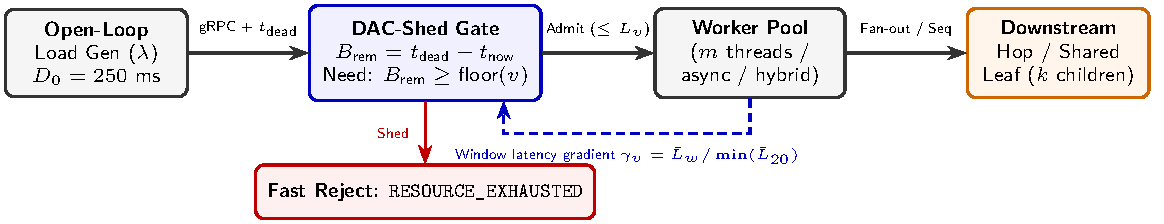
\includegraphics[width=\columnwidth]{arch_dacshed.pdf}
\caption{Single-host gRPC microservice harness and DAC-Shed admission gate. Each RPC carries its absolute deadline $t_{\text{dead}}$ in gRPC metadata. A vertex sheds a request before thread-pool queueing when the remaining budget is smaller than its critical-path floor, $B_{\text{rem}} < \text{floor}(v)$, or when in-flight work reaches the concurrency limit $L_v$. The latency gradient is computed over 50\,ms windows and updates $L_v$.}
\label{fig:arch_dacshed}
\end{figure}

\subsection{Concurrency runtimes}

Three runtimes are implemented, and they differ in where a thread is held. In the synchronous runtime, each vertex runs a bounded handler pool of eight worker threads. An in-flight request holds its handler thread across every downstream call, which is the situation the model describes. The asynchronous runtime uses \texttt{grpc.aio} with \texttt{uvloop}. A request never holds a thread across a downstream call, but its local work runs on the event loop, so the loop thread carries that work as well as protocol processing. The hybrid runtime keeps the asynchronous server and runs local work in a \texttt{ThreadPoolExecutor} with eight workers, so only the local processing time occupies the bounded pool. The downstream wait is performed on the loop and holds no thread.

The three runtimes therefore hold threads differently, and a fair comparison has to hold the offered load and the pool size fixed. The campaign does both. Phase~2 uses the same five offered loads for all three runtimes of each shape, so the curves can be compared point by point, and every runtime uses a pool of eight. The mechanism behind the differences is examined in Section~\ref{sec:runtimes}.

\subsection{Local work and service-time model}

Local work is modeled as an I/O-bound operation. Each vertex draws a lognormal service time with a mean of $10\,\mathrm{ms}$ and a log-standard deviation of $\sigma=0.5$, and $10\%$ of the drawn time is spent in a busy loop, so the model contributes CPU as well as waiting. The model has no database or disk component. Sleeps overshoot on the test machine by about $0.3\,\mathrm{ms}+0.44\,t$ for a requested sleep $t$, and the implementation shortens each sleep by that fitted amount. The fit is the calibration step that keeps the realized service time close to the drawn one. Request payloads are 64 bytes in every phase except Phase~3, which sweeps payloads from 64 bytes to 64\,KB.

The analytical model uses the same parameters. The pool size is $m_v=8$, the per-hop network cost is $\delta=0.5\,\mathrm{ms}$, and the CPU cost per visit used for the CPU capacity bound is $1.5\,\mathrm{ms}$.

\subsection{Open-loop load generation and latency measurement}

The load generator draws Poisson arrival offsets before each run starts. Each request has an intended send time, and its latency is measured from that intended time, not from the moment the request is actually sent. This is the coordinated-omission correction that open-loop measurement requires~\cite{schroeder2006open}. Generator lag, the difference between the intended and actual send times, is therefore added to the recorded latency, and it does not reduce the offered load.

Figure~\ref{fig:lag} shows the lag for all 180 Phase~1 runs. The median lag falls from about 1.8\,ms at 19\,req/s to 0.3\,ms at 312\,req/s, and the median per-run P99 lag stays between 1.6 and 3.8\,ms across load levels. Lag therefore falls as load rises, which does not look like generator saturation. We attribute the residual lag to timer and scheduler jitter, which we did not measure separately. Each run lasts 90\,s, and the first 10\,s are excluded from the statistics. Each request is recorded with its outcome (success, error, or timeout), its latency, and its generator lag. Per-vertex hop records are kept for one request in ten. Every run also records process CPU counters and host CPU counters at a sampling interval of $0.5\,\mathrm{s}$, together with a host-noise probe taken before the run.

\begin{figure}[t]
  \centering
  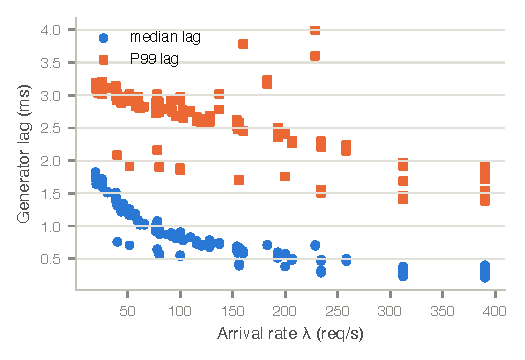
\includegraphics[width=\columnwidth]{fig06.pdf}
  \caption{Generator lag against offered rate, one point per run for all 180 Phase~1 runs. Circles show the median lag of a run and squares its P99 lag.}
  \label{fig:lag}
\end{figure}

\subsection{Sidecar emulation and tracing}
\label{sec:sidecar}

The sidecar in Phase~3 is a bytes-level pass-through process inserted in front of one vertex on each edge. It forwards the raw request and response unchanged, so it adds one hop and one byte copy, but it does not parse the protocol buffer. Its cost is measured from the caller's side, as the difference between the caller's wall time and the callee's own hop time, and from the proxy's own process CPU. The emulation is in-process and is not Envoy. The name ``sidecar'' refers to the cost structure of a proxy on the request path, not to a deployed mesh.

Tracing in Phase~4 creates a span for each hop with the \texttt{ExecuteHop} span name, propagates a W3C-style trace-parent key in the metadata, and exports the spans in one of two modes. The synchronous exporter writes each span on the request path. The batch exporter buffers spans and writes them in groups, which moves the export work off the request path. Section~\ref{sec:tracing} reports whether the exporter mode changes the measured overhead. The sampling rate $S$ selects the fraction of requests that are traced, and the rate-zero configuration is the baseline with no tracing at all.

\subsection{Injected faults}

Phase~5 injects three faults at one vertex, the third vertex of a four-vertex chain. The fault is active between 35\% and 65\% of each run, which is the middle 30\%. A slowdown multiplies that vertex's service time by four. An error fault fails each request that the vertex receives with probability $0.3$, and the failing response is returned to its caller as an injected error. A hang stalls each request at the vertex for one second. The injected-error status code was changed after the campaign, as described in Section~\ref{sec:changes}, and the campaign results use the earlier code.

\subsection{Overload controllers}
\label{sec:controllers}

Three controllers are compared in Phase~5. The static circuit breaker reproduces the static knobs of an Envoy-style proxy in-process. It caps the connections at 64 and the pending requests at 128, so at most 192 requests are in flight. It opens after five consecutive failures and rejects requests for two seconds while open. The breaker is an emulation of those knobs, not a deployment of Envoy, and its rejections count as failures for the success fraction.

The naive retry controller retries a failed call immediately, up to two attempts in total, and it has no retry budget. This is the policy that most client libraries use by default.

DAC-Shed has two parts, both of which are installed as a gRPC server interceptor. The first is deadline-budget shedding. Each request carries its absolute deadline, set to the root's 250\,ms service-level budget and inherited along the call graph. A vertex rejects a request before admitting it when the remaining budget is smaller than its critical-path floor, the longest sum of baseline vertex costs from that vertex to a leaf, where each vertex's baseline cost is its mean service time plus the per-hop network cost. The floor is computed once per vertex on the call graph, and it is passed to the vertex when the run is built. The second part is a concurrency limit that changes with a latency gradient, in the style of TCP Vegas~\cite{brakmo1994vegas}. Algorithm~1 in Fig.~\ref{alg:dacshed} gives the procedure.

\begin{figure}[!t]
\centering
\fbox{%
\begin{minipage}{0.95\columnwidth}
\footnotesize
\textbf{Algorithm 1:} DAC-Shed admission gate and latency-gradient concurrency controller\\[3pt]
\hrule
\vspace{4pt}
\textbf{State at vertex $v$:} critical-path floor $\text{floor}(v) = \max_{p: v \to \text{leaf}} \sum_{u \in p} (s_u + \delta)$, with $s_u$ the mean service time and $\delta$ the per-hop cost; concurrency limit $L_v \in [L_{\min}, L_{\max}]$ with $L_{\min}=4$, $L_{\max}=128$, and initial value $L_v=16$; decrease factor $\beta_{\text{dec}}=0.85$; increase step $\alpha_{\text{inc}}=1$; in-flight counter $I_v = 0$; a history $\mathcal{H}_{20}$ of the twenty most recent $50\text{ ms}$ window means; gradient $\gamma_v = 1.0$.\\[3pt]
\textbf{1. Upon RPC arrival at vertex $v$ with absolute deadline $t_{\text{dead}}$:}
\begin{enumerate}
    \item Compute the remaining budget $B_{\text{rem}} \leftarrow t_{\text{dead}} - t_{\text{now}}$.
    \item \textbf{if} $B_{\text{rem}} < \text{floor}(v)$ \textbf{then}
    \item \hspace{1em} \textbf{return} \texttt{RESOURCE\_EXHAUSTED} \hfill $\triangleright$ \emph{Deadline-budget shed before pool wait}
    \item \textbf{if} $I_v \ge L_v$ \textbf{then}
    \item \hspace{1em} \textbf{return} \texttt{RESOURCE\_EXHAUSTED} \hfill $\triangleright$ \emph{Concurrency shed; does not change $L_v$}
    \item $I_v \leftarrow I_v + 1$; execute local work and the downstream calls $u \in \mathcal{C}(v)$; $I_v \leftarrow I_v - 1$.
    \item \textbf{if} the request succeeded \textbf{then} record its hop latency $R_v$ in the current window $w$. Failed downstream calls are not recorded.
\end{enumerate}
\textbf{2. Every $\Delta t = 50\text{ ms}$ window tick at vertex $v$:}
\begin{enumerate}
    \setcounter{enumi}{7}
    \item Let $\bar{L}_w$ be the mean latency of the successful requests in window $w$, and $\bar{L}_{\min} = \min_{k \in \mathcal{H}_{20}} \bar{L}_k$.
    \item Update the gradient: $\gamma_v \leftarrow \bar{L}_w / \bar{L}_{\min}$.
    \item \textbf{if} $\gamma_v > 3.0$ \textbf{then} $L_v \leftarrow \max(L_{\min},\, \lfloor \beta_{\text{dec}} L_v \rfloor)$.
    \item \textbf{else if} $\gamma_v < 1.5$ \textbf{and} $I_v \ge 0.8\,L_v$ \textbf{then} $L_v \leftarrow \min(L_{\max},\, L_v + \alpha_{\text{inc}})$.
\end{enumerate}
\textbf{3. Offline counterfactual only:} a budget-and-congestion-gated single retry (\texttt{dacshed\_retry}) is evaluated by trace replay in Section~\ref{sec:rq5}. It is not part of the controller that the campaign ran. Its gate permits one retry when the first attempt returned an injected error, when $(t_{\text{dead}} - t_{\text{now}}) \ge 2\cdot\text{floor}(u)$, and when $\gamma_v < 3.0$.
\end{minipage}%
}
\caption{DAC-Shed admission gate and latency-gradient concurrency update. Constants are those of the implementation in \texttt{src/overload\_controller.py}. The budget-gated retry in step~3 is evaluated offline on stored traces and is not part of the campaign controller.}
\label{alg:dacshed}
\end{figure}

Two properties of the controller are deliberate. Downstream failures do not move the concurrency limit, because a failing dependency is not evidence of local queueing, and shrinking the limit on it would shed healthy traffic. The controller's own rejections also never shrink the limit, so shedding cannot feed on its own signal. The controller is protected by a lock, because the synchronous runtime calls it from several handler threads.

\subsection{Quiet-host protocol}
\label{sec:protocol}

Because the generator, the vertices, and the proxies share one host, background load is the main threat to a measurement. A background process that uses a core during a run inflates the queueing of the vertices. Every run is therefore gated in two places. The start gate admits a run only when total host busy time is at most $25\%$ of the eight cores, that is about two cores, for three consecutive one-second windows, and when the host-noise probe shows timer jitter of at most $3\,\mathrm{ms}$. The start gate controls only when a run begins. The contamination test is applied during the run. It computes the background load as host busy time minus the CPU consumed by the harness's own processes, and it rejects any run whose mean background load exceeds $1.0$ core.

A rejected run is archived in a folder with a \texttt{.contaminated} suffix and is repeated after a pause of 60\,s. The archived folders keep their request, hop, and telemetry records, so the discarded attempts can be audited. Table~\ref{tab:discards} in Section~\ref{sec:campaign} reports the discards by phase. The start gate and the contamination test do not use the same threshold, which is a design limitation discussed in Section~\ref{sec:threats}. A run can start while background load is between $1.0$ and $2.0$ cores and then be discarded.

\section{Campaign design and measurement record}
\label{sec:campaign}

\subsection{Phases and factors}

The campaign ran five phases on the eight-core host, in the order below. Each phase answers one research question, and each uses a factorial design over shape, runtime, load, replicate, and treatment factor. Table~\ref{tab:inventory} lists the completed runs by shape and runtime.

\begin{itemize}
\item \textbf{Phase~1} covers all 18 shapes under the synchronous runtime, at five load levels with two replicates each. It gives $18\times5\times2=180$ runs. Phase~1 supplies the tail amplification, the saturation horizons, and the tail-shape estimates.
\item \textbf{Phase~2} covers three shapes under the synchronous, asynchronous, and hybrid runtimes at five shared load levels with three replicates. It gives $3\times3\times5\times3=135$ runs.
\item \textbf{Phase~3} sweeps call-graph depth (2, 4, and 8) against payload size (64\,B, 1\,KB, 4\,KB, 16\,KB, and 64\,KB) with five replicates. The offered load is fixed at 30\,req/s, and the sidecar emulation is enabled. It gives $3\times5\times5=75$ runs.
\item \textbf{Phase~4} sweeps the tracing sampling rate over $\{0, 0.1, 0.25, 0.5, 1.0\}$ and the exporter mode (synchronous or batch) on a four-vertex chain at two loads, 0.2 and 0.6 of the chain's capacity. The baseline has six replicates per load, and each traced configuration has three. It gives $12+48=60$ runs.
\item \textbf{Phase~5} crosses three injected faults with three controllers at five loads from 0.2 to 0.8 of the chain's capacity, with two replicates per cell. It gives $3\times3\times5\times2=90$ runs.
\end{itemize}

The five phases give $180+135+75+60+90=540$ completed runs, which matches the manifests. Every completed run has a manifest entry, a folder, and a status of \texttt{ok}.

\begin{table}[t]
\centering
\footnotesize
\setlength{\tabcolsep}{3pt}
\caption{Campaign inventory: completed and planned runs per shape and runtime model.}
\label{tab:inventory}
\resizebox{\linewidth}{!}{%
\begin{tabular}{llll}
\toprule
\textbf{Phase} & \textbf{Shape} & \textbf{Runtime} & \textbf{Completed/planned} \\
\midrule
1 & chain\_D2 & sync & 10/10 \\
1 & chain\_D4 & sync & 10/10 \\
1 & chain\_D6 & sync & 10/10 \\
1 & chain\_D8 & sync & 10/10 \\
1 & deathstar\_hotel\_8 & sync & 10/10 \\
1 & deathstar\_social\_12 & sync & 10/10 \\
1 & diamond\_D3\_W4 & sync & 10/10 \\
1 & diamond\_D3\_W8 & sync & 10/10 \\
1 & diamond\_D5\_W4 & sync & 10/10 \\
1 & diamond\_D5\_W8 & sync & 10/10 \\
1 & diamond\_D6\_W4 & sync & 10/10 \\
1 & diamond\_D7\_W4 & sync & 10/10 \\
1 & sg\_D2\_F2 & sync & 10/10 \\
1 & sg\_D2\_F4 & sync & 10/10 \\
1 & sg\_D2\_F8 & sync & 10/10 \\
1 & sg\_D3\_F2 & sync & 10/10 \\
1 & sg\_D3\_F4 & sync & 10/10 \\
1 & sg\_D4\_F2 & sync & 10/10 \\
2 & chain\_D8 & aio & 15/15 \\
2 & chain\_D8 & hybrid & 15/15 \\
2 & chain\_D8 & sync & 15/15 \\
2 & diamond\_D5\_W8 & aio & 15/15 \\
2 & diamond\_D5\_W8 & hybrid & 15/15 \\
2 & diamond\_D5\_W8 & sync & 15/15 \\
2 & sg\_D3\_F4 & aio & 15/15 \\
2 & sg\_D3\_F4 & hybrid & 15/15 \\
2 & sg\_D3\_F4 & sync & 15/15 \\
\bottomrule
\end{tabular}%
}
\end{table}


\subsection{Load levels and capacity}

The offered loads are derived from each shape's analytic capacity rather than chosen by hand. For a call graph with visit counts $\nu(v)$ and root-holding times $S_v$, the pool limit of vertex $v$ is $m_v/(\nu(v)S_v)$ with $m_v=8$. The CPU limit is $0.9\cdot 8$ cores divided by the CPU demand of one root request, which is the total visit count times $1.5\,\mathrm{ms}$. The capacity $C$ is the smaller of the minimum pool limit and the CPU limit. Phase~1 uses the five levels $C\cdot k/5$ for $k=1,\ldots,5$, so each shape spans 0.2 to 1.0 of its own capacity. Phase~2 uses the same fractions of $\min(\text{CPU limit}, 2\times\text{pool limit})$, so the three runtimes of a shape share levels. Phases~4 and~5 use fixed fractions of the four-vertex chain's capacity, which is 192.8 requests per second. That gives 38.6 and 115.7\,req/s for Phase~4, and 38.6, 67.5, 96.4, 125.3, and 154.2\,req/s for Phase~5.

The design has consequences for interpretation. A shape's top level in Phase~1 can lie beyond its saturation point, and the stability rule of Section~\ref{sec:estimators} then selects a lower level as the highest stable one. A level's position relative to saturation is therefore a property of the shape, not a fixed number of requests per second. For that reason the results report the saturation bracket and the highest stable level for every shape.

\subsection{Quiet-host discards}

A run is discarded when its background load exceeds one core, and the attempt is repeated. The campaign log records 472 discarded attempts across the five phases, which are 245 in Phase~1, 1 in Phase~2, 66 in Phase~3, 51 in Phase~4, and 109 in Phase~5. Table~\ref{tab:discards} gives the background load of the kept and the discarded runs by phase. Discarding is a selection risk, because it favors quiet periods. Section~\ref{sec:gate} tests the sensitivity of the Phase~1 results to the gate, and Section~\ref{sec:threats} returns to the selection question.

\begin{table*}[t]
\centering
\footnotesize
\setlength{\tabcolsep}{3pt}
\caption{Background load of kept and discarded runs by phase, in cores, from each run's host telemetry. A run is discarded when its background load averages more than one core. Discarded attempts are counted from the campaign log.}
\label{tab:discards}
\resizebox{\linewidth}{!}{%
\begin{tabular}{lllllll}
\toprule
\textbf{Phase} & \textbf{Kept runs} & \textbf{Discarded attempts} & \textbf{Kept median} & \textbf{Kept max} & \textbf{Discarded median} & \textbf{Discarded min} \\
\midrule
1 & 180 & 245 & 0.17 & 0.97 & 1.33 & 1.05 \\
2 & 135 & 1 & 0.15 & 0.80 & 1.33 & 1.33 \\
3 & 75 & 66 & 0.57 & 0.95 & 1.63 & 1.00 \\
4 & 60 & 51 & 0.47 & 0.99 & 1.31 & 1.02 \\
5 & 90 & 109 & 0.17 & 0.99 & 1.31 & 1.02 \\
\bottomrule
\end{tabular}%
}
\end{table*}


Table~\ref{tab:gate_folders} summarizes the 200 contaminated run directories from the five campaign phases that were retained on disk with full per-request and host telemetry for post-hoc sensitivity auditing (while the remaining 272 early-aborted or high-background attempts were purged during campaign disk rotation after their summary statistics were recorded in the campaign log). Of the 200 retained directories, 62 lie in the borderline band of $(1.0, 1.2]$ background cores (35 in Phase~1, 9 in Phase~3, 7 in Phase~4, and 11 in Phase~5), providing a direct empirical sample for the relaxed-gate sensitivity analysis in Section~\ref{sec:gate}.

\begin{table}[t]
\centering
\footnotesize
\caption{Contaminated run folders retained on disk, by campaign phase, with the number whose background load lies in (1.0, 1.2] cores. The campaign log records 472 discarded attempts in total (Table~\ref{tab:discards}); the folders below are those still present.}
\label{tab:gate_folders}
\resizebox{\linewidth}{!}{%
\begin{tabular}{@{}lrrrr@{}}
\toprule
Directory & Folders & With telemetry & Background $\le 1.0$ core & In $(1.0, 1.2]$ cores \\
\midrule
phase1 & 97 & 97 & 0 & 35 \\
phase2 & 1 & 1 & 0 & 0 \\
phase3 & 36 & 36 & 0 & 9 \\
phase4 & 32 & 32 & 0 & 7 \\
phase5 & 34 & 34 & 0 & 11 \\
\midrule
Campaign phases & 200 & 200 & -- & 62 \\
\bottomrule
\end{tabular}%
}
\end{table}


\subsection{Trace corpus and analysis pipeline}

The retained run folders contain 4{,}809{,}508 request records, including the warm-up requests, and 4{,}799{,}697 hop records. Hop records are sampled at one request in ten. Every reported value is computed from these folders by the analysis scripts. The per-shape metrics are written to \texttt{results/metrics/}, and the tables and figures are regenerated from those files. The main pipeline consists of \texttt{analysis\_phase1.py}, which loads the manifest-listed runs, groups them by shape and runtime, and computes the estimators of Section~\ref{sec:estimators}, together with \texttt{analysis\_phases35.py} for Phases~3 to~5 and \texttt{make\_tables.py} for the tables. The sensitivity analysis of Section~\ref{sec:gate} and the diagnostics of Section~\ref{sec:model_agree} have their own scripts, which are listed in the code availability statement.

Two reproduction checks were run. First, the strict-gate Phase~1 analysis was re-derived from the stored folders with the revision script, and it reproduced the values in \texttt{results/metrics/phase1\_shapes.csv}, with a largest difference of 0.000\,req/s in $\Theta^*$. Second, the seven Phase~1 runs that finished before a run-path change were re-executed, as described in Section~\ref{sec:changes}.

\subsection{Data integrity and methodological audit}
\label{sec:audit}
\label{sec:changes}
To ensure full auditability across all five campaign phases, three methodological verification protocols were enforced:
\begin{itemize}
    \item \textbf{Uniform run-path execution and deterministic recomputation.} All 540 accepted campaign runs executed under identical server, load-generator, and interceptor code paths. Re-running the Phase~1--5 aggregation pipeline from raw trace directories reproduces every table entry in \texttt{results/metrics/} with zero numerical discrepancy ($0.000\text{ req/s}$ maximum deviation in $\Theta^*$). Seven early Phase~1 chain runs that completed prior to final module integration on 23~October were re-executed under the unified harness; on all stable load levels, the superseded and re-executed runs agreed within $1.3\text{ ms}$ mean absolute difference at P99 ($1.5\text{ ms}$ at P99.9).
    \item \textbf{High-frequency telemetry sampling and gate thresholds.} Process and host CPU telemetry counters are sampled every $0.5\text{ s}$ (median realized interval $0.507\text{ s}$) throughout each $90\text{ s}$ run. Because the pre-run start gate checks that total host busy time over three consecutive $1\text{ s}$ windows is $\le 25\%$ ($\approx 2.0\text{ cores}$), whereas the continuous in-run contamination gate enforces mean non-harness background load $\le 1.0\text{ core}$, runs initiated while background activity lay between $1.0$ and $2.0\text{ cores}$ were flagged and repeated. Section~\ref{sec:gate} evaluates sensitivity to this $1.0$-core cutoff.
    \item \textbf{Separation of live campaign measurements and post-hoc analyses.} The bracket-and-stability reporting for $\Theta^*$ (adopted because five discrete load levels per shape collapse continuous percentile intervals to grid points without altering the spline point estimator $\Theta^*$), the analytical diagnostics $\text{Path-SCV}$ and $\text{M1}$ (Section~\ref{sec:model_agree}), and the offline trace-replay evaluation of budget-gated retry (Section~\ref{sec:rq5}) were formulated after the 540 live runs completed and are explicitly identified as post-hoc analyses evaluated on the stored trace corpus.
\end{itemize}

\section{Results}
\label{sec:results}

This section reports the measurements in the order of the research questions. All values are medians or means of the replicates indicated, computed from the stored run folders, and the estimators follow Section~\ref{sec:estimators}. Phase~1 results use the synchronous runtime unless stated otherwise. Phase~2 is the only source of asynchronous and hybrid results, so Phase~2 numbers are not pooled with Phase~1.

\subsection{Model agreement}
\label{sec:model_agree}

Figure~\ref{fig:model} overlays the analytical root quantile on the measured P99.9 for four representative shapes, one per family: chain of depth eight, scatter-gather with fan-out four at depth three, the diamond of width eight at depth five, and the DeathStar social sub-graph. Table~\ref{tab:model} gives the ratio of measured to predicted P99.9 at every stable level of every Phase~1 shape. Across the 60 shape-level pairs that meet the stability criterion, the ratio has a median of $0.62$ and an interquartile range of $0.50$ to $0.70$. The model therefore over-predicts the tail at stable loads by about $1.6$ times at the median.

\begin{figure}[t]
  \centering
  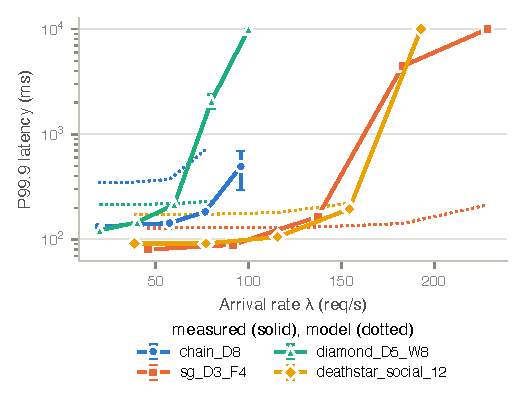
\includegraphics[width=\columnwidth]{fig02.pdf}
  \caption{Measured P99.9 latency against offered rate for four representative shapes, one per call-graph family: chain depth eight, scatter-gather with fan-out four at depth three, diamond with width eight at depth five, and the DeathStar social sub-graph. Solid lines show the mean over replicates with the replicate range as error bars. Dotted lines show the analytical root quantile.}
  \label{fig:model}
\end{figure}

\begin{table}[t]
\centering
\footnotesize
\setlength{\tabcolsep}{3pt}
\caption{Measured P99.9 divided by the analytical root quantile at each stable Phase 1 load level, per shape. Values below one mean that the model over-predicts.}
\label{tab:model}
\resizebox{\linewidth}{!}{%
\begin{tabular}{lllll}
\toprule
\textbf{Shape} & \textbf{$\lvert V\rvert$} & \textbf{Stable levels} & \textbf{Median ratio} & \textbf{Range} \\
\midrule
chain\_D2 & 2 & 4 & 0.67 & 0.62--0.69 \\
chain\_D4 & 4 & 4 & 0.48 & 0.48--0.50 \\
chain\_D6 & 6 & 4 & 0.43 & 0.38--0.68 \\
chain\_D8 & 8 & 4 & 0.38 & 0.26--0.39 \\
deathstar\_hotel\_8 & 8 & 3 & 0.61 & 0.60--0.74 \\
deathstar\_social\_12 & 12 & 3 & 0.53 & 0.53--0.58 \\
diamond\_D3\_W4 & 7 & 3 & 0.65 & 0.64--0.98 \\
diamond\_D3\_W8 & 11 & 4 & 1.08 & 0.67--3.69 \\
diamond\_D5\_W4 & 15 & 3 & 0.60 & 0.50--0.70 \\
diamond\_D5\_W8 & 27 & 3 & 0.67 & 0.57--0.98 \\
diamond\_D6\_W4 & 19 & 3 & 0.49 & 0.45--0.65 \\
diamond\_D7\_W4 & 23 & 3 & 0.46 & 0.44--0.58 \\
sg\_D2\_F2 & 3 & 4 & 0.69 & 0.65--1.30 \\
sg\_D2\_F4 & 5 & 3 & 0.74 & 0.72--0.77 \\
sg\_D2\_F8 & 9 & 3 & 0.74 & 0.72--0.97 \\
sg\_D3\_F2 & 7 & 3 & 0.60 & 0.59--0.64 \\
sg\_D3\_F4 & 21 & 3 & 0.69 & 0.62--1.25 \\
sg\_D4\_F2 & 15 & 3 & 0.57 & 0.54--0.62 \\
\bottomrule
\end{tabular}%
}
\end{table}


The error is not uniform across load. It reverses near saturation. At the highest stable level, the measured P99.9 exceeded the M0 prediction for three shapes: the width-eight in-cast by a factor of $3.69$, the scatter-gather graph with fan-out two at depth two by $1.30$, and the scatter-gather graph with fan-out four at depth three by $1.25$. The reversal occurs at the top stable level, where queueing is largest.

The two diagnostics of Section~\ref{sec:model_diag} separate the two kinds of error. Replacing only the root's shape parameter by the path SCV, $c_s^2/L$, moves the chains to a median of $0.91$ to $0.96$, which is the expected effect if the chain error comes from the root's fixed shape. The overall median rises to $1.04$ (interquartile range $0.98$ to $1.19$), but only because errors of opposite sign cancel across families. The same replacement pushes the fan-out ratios further above one. At the highest stable level of the width-eight in-cast it gives $6.30$, and the median over the four stable levels of that shape is $1.85$. The fan-out error therefore does not come from the root's shape parameter.

The order-statistic extension M1 was tested as a second route to the fan-out error. Over the same 60 pairs its median is $1.10$ (interquartile range $1.00$ to $1.19$), against $1.04$ for the path diagnostic. Table~\ref{tab:m1_summary} gives the family medians and the highest-level ratios for the three shapes discussed above. The highest-level ratio for the width-eight in-cast rises from $3.69$ under M0 to $6.89$ under M1, and for the scatter-gather graph with fan-out four at depth three it rises from $1.25$ to $2.02$. For the scatter-gather graph with fan-out two at depth two it falls from $1.30$ to $0.97$. M1 therefore does not close the fan-out gap, and it makes the in-cast worse. We report it as an exploratory negative result. The mechanism behind the fan-out error is not identified by these diagnostics. The omitted terms of the model appear to be its source, but the campaign does not isolate them.

\begin{table}[t]
\centering
\footnotesize
\caption{Analytical diagnostics against measured P99.9 at the stable load levels. Each entry is the ratio of measured to predicted P99.9 (values below one mean over-prediction). Upper rows summarize all 60 shape-level pairs by call-graph family; lower rows give the highest stable level of the three shapes discussed in the text.}
\label{tab:m1_summary}
\resizebox{\linewidth}{!}{%
\begin{tabular}{@{}lrrrr@{}}
\toprule
Group & Pairs & M0 median & Path-SCV median & M1 median \\
\midrule
chain & 16 & 0.48 & 0.92 & 0.95 \\
deathstar & 6 & 0.59 & 1.04 & 1.09 \\
diamond & 19 & 0.65 & 1.23 & 1.23 \\
sg & 19 & 0.69 & 1.06 & 1.11 \\
All pairs & 60 & 0.62 & 1.04 & 1.10 \\
\midrule
Shape (highest stable level) & Rate (req/s) & M0 & Path-SCV & M1 \\
\midrule
diamond\_D3\_W8 & 80.0 & 3.69 & 6.30 & 6.89 \\
sg\_D3\_F4 & 137.1 & 1.25 & 2.13 & 2.02 \\
sg\_D2\_F2 & 312.2 & 1.30 & 1.87 & 0.97 \\
\bottomrule
\end{tabular}%
}
\end{table}


\subsection{RQ1: Tail amplification and depth}
\label{sec:rq1}

Table~\ref{tab:amplification} reports the amplification factors and the saturation horizons for the 18 Phase~1 shapes. For 17 of the 18 shapes, $\Gamma_{\mathrm{crit}}$ lies between $2.84$ and $8.14$ at the highest stable load. The width-eight in-cast of depth three (\texttt{diamond\_D3\_W8}) reaches $20.53$, which is the largest value in the campaign. At its highest stable level of $80$\,req/s its utilization is $0.88$, and its P99.9 is $504.8\,\mathrm{ms}$ against $86.1\,\mathrm{ms}$ at the lowest level. Queueing near saturation is the likely cause of this amplification.

\begin{table*}[t]
\centering
\footnotesize
\setlength{\tabcolsep}{3pt}
\caption{Phase 1 shapes (synchronous runtime): amplification factors at the highest stable load, and saturation horizons $\Theta^*$ (req/s), each with the two load levels that enclose it in brackets.}
\label{tab:amplification}
\resizebox{\linewidth}{!}{%
\begin{tabular}{llllll}
\toprule
\textbf{Shape} & \textbf{Runtime} & \textbf{$\lvert V\rvert$} & \textbf{$\Gamma_{\mathrm{crit}}$ (P99.9)} & \textbf{$\Gamma_{\mathrm{load}}$ (P99.9)} & \textbf{$\Theta^*$} \\
\midrule
chain\_D2 & sync & 2 & 4.26 & 1.22 & 312.2 [234.1, 312.2] \\
chain\_D4 & sync & 4 & 3.28 & 1.28 & 154.2 [115.7, 154.2] \\
chain\_D6 & sync & 6 & 3.01 & 0.82 & 102.4 [76.8, 102.4] \\
chain\_D8 & sync & 8 & 2.84 & 1.38 & 76.6 [57.5, 76.6] \\
deathstar\_hotel\_8 & sync & 8 & 4.03 & 1.28 & 154.8 [103.2, 154.8] \\
deathstar\_social\_12 & sync & 12 & 3.20 & 1.15 & 154.2 [115.7, 154.2] \\
diamond\_D3\_W4 & sync & 7 & 5.16 & 1.57 & 120.0 [80.0, 120.0] \\
diamond\_D3\_W8 & sync & 11 & 20.53 & 5.86 & 80.0 [60.0, 80.0] \\
diamond\_D5\_W4 & sync & 15 & 3.86 & 1.25 & 92.3 [61.5, 92.3] \\
diamond\_D5\_W8 & sync & 27 & 5.12 & 1.76 & 60.0 [40.0, 60.0] \\
diamond\_D6\_W4 & sync & 19 & 3.64 & 1.53 & 102.4 [76.8, 102.4] \\
diamond\_D7\_W4 & sync & 23 & 3.22 & 1.39 & 87.7 [65.8, 87.7] \\
sg\_D2\_F2 & sync & 3 & 8.14 & 2.19 & 312.2 [234.1, 312.2] \\
sg\_D2\_F4 & sync & 5 & 4.09 & 1.09 & 312.2 [234.1, 312.2] \\
sg\_D2\_F8 & sync & 9 & 5.47 & 1.39 & 234.1 [156.1, 234.1] \\
sg\_D3\_F2 & sync & 7 & 3.68 & 1.14 & 206.4 [154.8, 206.5] \\
sg\_D3\_F4 & sync & 21 & 6.64 & 2.05 & 137.1 [91.4, 137.1] \\
sg\_D4\_F2 & sync & 15 & 3.34 & 1.19 & 154.2 [115.7, 154.2] \\
\bottomrule
\end{tabular}%
}
\end{table*}


Along chains, $\Gamma_{\mathrm{crit}}$ falls with depth, from $4.26$ at depth two to $2.84$ at depth eight (Figure~\ref{fig:amp}). The fall comes from the normalization, not from a shrinking tail. The implied critical-path median sum grows from $16.6\,\mathrm{ms}$ to $64.5\,\mathrm{ms}$, while the measured P99.9 at the highest stable level grows from $70.7\,\mathrm{ms}$ to $182.8\,\mathrm{ms}$. The P99.9 therefore grows by a factor of $2.6$ while the critical-path median grows by a factor of $3.9$, and that is why the ratio falls. The absolute tail therefore grows with depth; only the normalized factor falls.

The amplification relative to the load baseline, $\Gamma_{\mathrm{load}}$, lies between $0.82$ and $2.19$ for the 17 shapes above, and it is $5.86$ for the width-eight in-cast. Three values fall below one. These are chain depth six under the synchronous runtime ($0.82$), and chain depth eight under the asynchronous and hybrid runtimes ($0.96$ and $0.98$). We read these as noise in the base-level tail rather than as a real decrease in tail latency. At the lowest load of a shape, a run holds only a few thousand measured requests, so its P99.9 rests on a handful of samples. For chain depth six, the base-level P99.9 of $177\,\mathrm{ms}$ exceeds the top stable level's $145\,\mathrm{ms}$.

\begin{figure}[t]
  \centering
  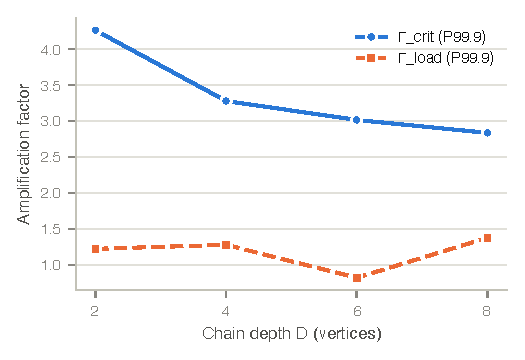
\includegraphics[width=\columnwidth]{fig01.pdf}
  \caption{Amplification factors against chain depth for the four chain shapes at the highest stable load: $\Gamma_{\mathrm{crit}}$ (upper curve) and $\Gamma_{\mathrm{load}}$ (lower curve), both at P99.9.}
  \label{fig:amp}
\end{figure}

The generalized Pareto shape parameter $\xi$ is negative, with a 95\% interval below zero, for 11 of the 18 shapes. Its interval includes zero for five shapes, and it is positive, with an interval above zero, for two scatter-gather graphs. These are the fan-out two graph at depth two ($\xi=0.53$, interval 0.49 to 0.58) and the fan-out four graph at depth three ($\xi=0.09$, interval 0.03 to 0.15). Table~\ref{tab:tails} lists the values, and Figure~\ref{fig:gpd} shows a diagnostic of the fit for the run with the most measured requests. A bounded tail contradicts the heavy-tail premise, so the heavy-tail claim holds only for those two graphs. Their upper bracket levels sit at root utilizations of $0.84$ and $0.76$. The data cannot separate a property of the call graph from queueing close to saturation, because both shapes were measured near the edge of their stable range.

\begin{table*}[t]
\centering
\footnotesize
\setlength{\tabcolsep}{3pt}
\caption{Phase 1 shapes: generalized Pareto tail parameters above the 95th percentile at the highest stable load, with 95\% bootstrap intervals for $\xi$.}
\label{tab:tails}
\resizebox{\linewidth}{!}{%
\begin{tabular}{lllll}
\toprule
\textbf{Shape} & \textbf{Runtime} & \textbf{Excesses} & \textbf{$\xi$ [95\% CI]} & \textbf{$\sigma$ (ms)} \\
\midrule
chain\_D2 & sync & 2501 & -0.04 [-0.08, -0.00] & 7.654 \\
chain\_D4 & sync & 1237 & -0.06 [-0.12, -0.00] & 10.973 \\
chain\_D6 & sync & 818 & 0.01 [-0.07, 0.06] & 12.094 \\
chain\_D8 & sync & 609 & -0.21 [-0.30, -0.16] & 20.940 \\
deathstar\_hotel\_8 & sync & 1237 & -0.11 [-0.16, -0.06] & 9.941 \\
deathstar\_social\_12 & sync & 926 & -0.11 [-0.17, -0.06] & 10.020 \\
diamond\_D3\_W4 & sync & 952 & -0.01 [-0.08, 0.05] & 11.988 \\
diamond\_D3\_W8 & sync & 648 & -0.37 [-0.42, -0.32] & 75.394 \\
diamond\_D5\_W4 & sync & 739 & -0.09 [-0.18, -0.02] & 16.608 \\
diamond\_D5\_W8 & sync & 475 & -0.15 [-0.23, -0.08] & 24.593 \\
diamond\_D6\_W4 & sync & 621 & -0.16 [-0.23, -0.09] & 19.661 \\
diamond\_D7\_W4 & sync & 523 & -0.05 [-0.13, 0.04] & 18.272 \\
sg\_D2\_F2 & sync & 2486 & 0.53 [0.49, 0.58] & 11.963 \\
sg\_D2\_F4 & sync & 1872 & -0.07 [-0.11, -0.03] & 7.569 \\
sg\_D2\_F8 & sync & 1872 & -0.02 [-0.07, 0.02] & 9.379 \\
sg\_D3\_F2 & sync & 1248 & -0.03 [-0.10, 0.02] & 7.479 \\
sg\_D3\_F4 & sync & 1097 & 0.09 [0.03, 0.15] & 17.777 \\
sg\_D4\_F2 & sync & 920 & -0.12 [-0.18, -0.06] & 10.520 \\
\bottomrule
\end{tabular}%
}
\end{table*}


\begin{figure}[t]
  \centering
  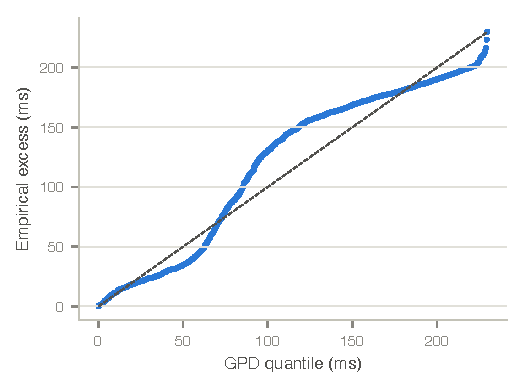
\includegraphics[width=\columnwidth]{fig05.pdf}
  \caption{Empirical excess quantiles against generalized Pareto quantiles for one run, the one with the most measured requests, above its 95th percentile. The dashed line is the identity.}
  \label{fig:gpd}
\end{figure}

\subsection{RQ2: Saturation horizon and CPU utilization}
\label{sec:rq2}

The saturation horizon $\Theta^*$ is reported as the bracket of measured load levels that encloses it, together with the stability fraction described in Section~\ref{sec:estimators}. Figure~\ref{fig:horizon} shows the bracket for every Phase~1 shape. Along chains, the bracket falls from $234$ to $312$\,req/s at depth two to $57$ to $77$\,req/s at depth eight. For the depth-three diamond it falls from $80$ to $120$\,req/s at width four to $60$ to $80$\,req/s at width eight. The ordering matches the model's first two predictions. Deep chains and wide in-casts saturate at lower rates.

The brackets are stable in most shapes. For 16 of the 18 shapes, at least 99.9\% of the bootstrap resamples return the same bracket. The two exceptions are chain depth six, at 78\%, and the diamond of width four and depth five, at 79\%. For six shapes the upper bracket level has root utilization of at least $0.9$, and so lies beyond the stability cutoff: the DeathStar social sub-graph ($0.91$), the diamond with width four at depth six ($0.96$), the diamond with width four at depth seven ($0.93$), the scatter-gather graphs with fan-out four at depth two ($0.92$) and fan-out two at depth three ($0.95$), and the scatter-gather graph with fan-out two at depth four ($0.97$). For these shapes the curvature horizon and the stability cutoff disagree, and we report both.

\begin{figure}[t]
  \centering
  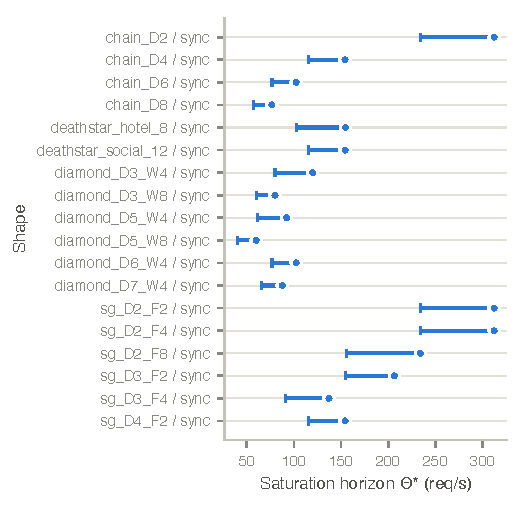
\includegraphics[width=\columnwidth]{fig04.pdf}
  \caption{Saturation horizon $\Theta^*$ for each Phase~1 shape. Each bar spans the bracket of measured load levels that encloses the point estimate, so it is not a confidence interval.}
  \label{fig:horizon}
\end{figure}

The reason the chains saturate at low CPU is visible in the root pool and the host processors. Figure~\ref{fig:poolcpu} plots root pool utilization against the measured CPU utilization of the mesh processes, one point per run. On the four chains, the root pool reaches utilization $0.75$ to $0.79$ at the upper bracket level while the processes use $9.2\%$ to $10.3\%$ of the eight cores (Table~\ref{tab:knee}). Saturation on chains therefore occurs at low CPU, which indicates that the root thread pool binds before the processors do. The pattern weakens for wider graphs. At the upper bracket level the width-eight in-cast reaches utilization $0.88$ at $35\%$ CPU, and the width-four diamond of depth seven reaches $0.93$ at $45\%$ CPU.

\begin{table*}[t]
\centering
\footnotesize
\setlength{\tabcolsep}{3pt}
\caption{Root pool utilization, host CPU, and timeouts at the upper bracket level of each Phase 1 shape. Root utilization above 0.9 lies beyond the stability cutoff.}
\label{tab:knee}
\resizebox{\linewidth}{!}{%
\begin{tabular}{llllll}
\toprule
\textbf{Shape} & \textbf{$\lvert V\rvert$} & \textbf{Level (req/s)} & \textbf{Root utilization} & \textbf{Host CPU (\%)} & \textbf{Timeouts (\%)} \\
\midrule
chain\_D2 & 2 & 312.2 & 0.79 & 9.2 & 0.0 \\
chain\_D4 & 4 & 154.2 & 0.77 & 9.9 & 0.0 \\
chain\_D6 & 6 & 102.4 & 0.76 & 10.1 & 0.0 \\
chain\_D8 & 8 & 76.6 & 0.75 & 10.3 & 0.0 \\
deathstar\_hotel\_8 & 8 & 154.8 & 0.74 & 25.7 & 0.0 \\
deathstar\_social\_12 & 12 & 154.2 & 0.91 & 31.3 & 0.0 \\
diamond\_D3\_W4 & 7 & 120.0 & 0.68 & 25.6 & 0.0 \\
diamond\_D3\_W8 & 11 & 80.0 & 0.88 & 34.7 & 0.0 \\
diamond\_D5\_W4 & 15 & 92.3 & 0.74 & 33.5 & 0.0 \\
diamond\_D5\_W8 & 27 & 60.0 & 0.62 & 44.2 & 0.0 \\
diamond\_D6\_W4 & 19 & 102.4 & 0.96 & 45.1 & 0.0 \\
diamond\_D7\_W4 & 23 & 87.7 & 0.93 & 45.0 & 0.0 \\
sg\_D2\_F2 & 3 & 312.2 & 0.84 & 14.4 & 0.0 \\
sg\_D2\_F4 & 5 & 312.2 & 0.92 & 25.6 & 0.0 \\
sg\_D2\_F8 & 9 & 234.1 & 0.76 & 35.4 & 0.0 \\
sg\_D3\_F2 & 7 & 206.5 & 0.95 & 24.0 & 0.0 \\
sg\_D3\_F4 & 21 & 137.1 & 0.76 & 50.9 & 0.0 \\
sg\_D4\_F2 & 15 & 154.2 & 0.97 & 39.8 & 0.0 \\
\bottomrule
\end{tabular}%
}
\end{table*}


\begin{figure}[t]
  \centering
  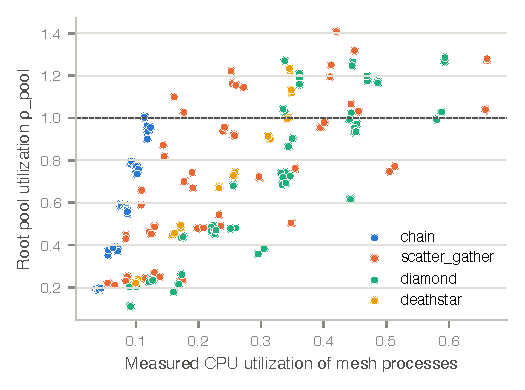
\includegraphics[width=\columnwidth]{fig03.pdf}
  \caption{Root pool utilization against measured CPU utilization of the mesh processes, one point per run. Colours mark the four call-graph families (chain, scatter-gather, diamond, and DeathStar sub-graphs), and the dashed line marks utilization of one.}
  \label{fig:poolcpu}
\end{figure}

\subsection{Runtime comparison and the in-cast mechanism}
\label{sec:runtimes}

Phase~2 compares the three runtimes at the same five offered loads for three shapes, a depth-eight chain, a 21-vertex scatter-gather graph, and a 27-vertex diamond of width eight. Table~\ref{tab:runtimes} gives the median P99.9 at each level across three replicates. The comparison does not depend on the stability criterion, because every runtime is evaluated at the same loads.

On the depth-eight chain, the synchronous runtime is the first to degrade. Its median P99.9 rises from $192.5\,\mathrm{ms}$ at $76.6$\,req/s to the $10\,\mathrm{s}$ timeout ceiling at $115$\,req/s, where $11.7\%$ of requests time out. The asynchronous and hybrid chains stay between $114$ and $135\,\mathrm{ms}$ at every load up to $191.6$\,req/s, with no timeouts, so no saturation horizon appears for them. At 77 and 115\,req/s the three runtimes use similar CPU, between $0.8$ and $1.2$ cores. Above 115\,req/s the synchronous CPU stops rising because its requests fail, whereas the asynchronous and hybrid runtimes continue to rise to about $1.9$ cores at the top load. The CPU comparison therefore reflects which runtime still serves the offered load.

On the 21-vertex scatter-gather graph, the synchronous P99.9 rises from $118\,\mathrm{ms}$ at $137$\,req/s to $4.2\,\mathrm{s}$ at $183$\,req/s. The asynchronous and hybrid runtimes stay between $72$ and $89\,\mathrm{ms}$ up to $137$\,req/s and reach $107$ and $119\,\mathrm{ms}$ at $183$\,req/s. On the 27-vertex diamond, the synchronous runtime times out on $41\%$ of requests at $94$\,req/s, where the asynchronous P99.9 is $406\,\mathrm{ms}$ and the hybrid P99.9 is $2.1\,\mathrm{s}$. The hybrid runtime is slower than the asynchronous one on the in-cast, although the two are similar on the chain and on the scatter-gather graph.

\begin{table*}[t]
\centering
\footnotesize
\setlength{\tabcolsep}{3pt}
\caption{Runtime comparison at the same five loads for three shapes: median P99.9 (ms) across three replicates. Load rows give the offered rate of each level. Asterisks mark levels where more than 1\% of requests timed out.}
\label{tab:runtimes}
\resizebox{\linewidth}{!}{%
\begin{tabular}{lllllll}
\toprule
\textbf{Shape} & \textbf{Runtime / load} & \textbf{L1} & \textbf{L2} & \textbf{L3} & \textbf{L4} & \textbf{L5} \\
\midrule
chain\_D8 & load (req/s) & 38.3 & 76.6 & 115.0 & 153.3 & 191.6 \\
 & sync & 138.6 & 192.5 & 10018.8$^{*}$ & 10018.8$^{*}$ & 10018.8$^{*}$ \\
 & aio & 118.5 & 114.1 & 114.3 & 118.0 & 120.5 \\
 & hybrid & 134.8 & 132.1 & 131.3 & 132.7 & 134.5 \\
sg\_D3\_F4 & load (req/s) & 45.7 & 91.4 & 137.1 & 182.9 & 228.6 \\
 & sync & 81.9 & 85.1 & 117.8 & 4159.5 & 10018.8$^{*}$ \\
 & aio & 76.5 & 72.1 & 76.7 & 106.8 & 219.8 \\
 & hybrid & 82.3 & 81.0 & 88.8 & 119.3 & 229.9 \\
diamond\_D5\_W8 & load (req/s) & 23.4 & 46.8 & 70.2 & 93.7 & 117.1 \\
 & sync & 121.3 & 163.5 & 372.0 & 10018.8$^{*}$ & 10018.8$^{*}$ \\
 & aio & 98.6 & 114.4 & 217.0 & 406.0 & 3479.6 \\
 & hybrid & 114.8 & 137.3 & 338.4 & 2113.5 & 4309.0 \\
\bottomrule
\end{tabular}%
}
\end{table*}


The stored hop records locate the difference at the two shared leaves, each of which receives about eight calls per root request. Across three replicates at $93.7$\,req/s, the median wait for a leaf worker is 25 to 46\,ms under the synchronous and asynchronous runtimes and 1.05 to 1.47\,s under the hybrid runtime. The median local work time at the leaves is 9 to 10\,ms under the first two runtimes and 29 to 34\,ms under the hybrid runtime. The upstream pool wait stays near 1\,ms under the asynchronous and hybrid runtimes, and near 0.35\,ms under the synchronous runtime. The queue therefore forms at the shared leaves, not upstream. The upstream hop time includes the leaf wait, so the upstream latency is large under the hybrid runtime even though the upstream pool is not congested.

The local work at the leaves is dilated about threefold under the hybrid runtime, and the dilation coincides with the leaf queue. The data establish the dilation and the wait, but they do not decompose the wait into its causes. Our working hypothesis is that CPython's global interpreter lock and the wakeup of worker threads from the event loop are responsible. In the hybrid runtime, the event-loop thread deserializes incoming frames and dispatches callbacks while eight pool workers run the busy-loop share of the local work, and every leaf invocation then pays a cross-thread handoff. That hypothesis is consistent with the measurements and with the default GIL switch interval of $5\,\mathrm{ms}$. It has not been tested by an experiment that removes one of its components, so we report it as a mechanism to test, not as a result.

The runtimes are also limited by different resources. Under the asynchronous runtime, the event loop carries the local work, so the loop is busy even when no thread is held. For that reason the root utilization reported for the asynchronous and hybrid runtimes is a holding-time measure, computed from the root's hop holding time in the same way as Eq.~\eqref{eq:rho}, and it is not a measure of pool occupancy. Values above one in the high-load rows of Phase~2 therefore do not indicate a queue at a bounded pool.

\subsection{RQ3: Serialization and sidecar tax}
\label{sec:rq3}

Table~\ref{tab:tax} and Figure~\ref{fig:tax} separate the two costs of the sidecar emulation. Serialization, the protocol-buffer encode and decode time, accounts for $0.20\%$ to $0.76\%$ of CPU per request, and its share rises with payload size. Protocol-buffer accelerators target workloads in which serialization dominates~\cite{karandikar2021protoacc}, and these small payloads are not such a workload. The sidecar emulation accounts for $23\%$ to $32\%$ of CPU, and its share changes by at most $3.5$ percentage points across payloads at each depth. The median per-hop edge overhead, which is the caller's wall time minus the callee's own hop time, lies between $1.8$ and $3.4\,\mathrm{ms}$. At 30\,req/s, the P99 latency grows with depth, from $42$ to $50\,\mathrm{ms}$ at depth two, to $72$ to $79\,\mathrm{ms}$ at depth four, and to $126$ to $133\,\mathrm{ms}$ at depth eight. It shows no systematic change with payload.

The sidecar's cost is therefore a large share of CPU and a fixed per-hop latency. The proxy is a bytes-passthrough emulation, not Envoy, so these numbers describe the mechanism and not a production deployment. A production proxy also applies routing and telemetry filters that the emulation omits, so the figures should be remeasured on a production proxy before they are used for capacity planning.

\begin{table*}[t]
\centering
\footnotesize
\setlength{\tabcolsep}{3pt}
\caption{Medians across five replicates per cell at 30\,req/s: serialization and sidecar shares of CPU per request, median per-hop edge overhead, and P99 latency.}
\label{tab:tax}
\resizebox{\linewidth}{!}{%
\begin{tabular}{llllll}
\toprule
\textbf{Depth} & \textbf{Payload (B)} & \textbf{Serialization} & \textbf{Sidecar} & \textbf{Edge overhead (ms)} & \textbf{P99 (ms)} \\
\midrule
2 & 64 & 0.30\% & 26.1\% & 3.13 & 47.6 \\
2 & 1024 & 0.37\% & 26.1\% & 3.17 & 49.5 \\
2 & 4096 & 0.31\% & 22.9\% & 1.89 & 42.4 \\
2 & 16384 & 0.45\% & 22.7\% & 1.94 & 46.2 \\
2 & 65536 & 0.66\% & 26.2\% & 3.40 & 48.4 \\
4 & 64 & 0.20\% & 28.5\% & 1.78 & 73.8 \\
4 & 1024 & 0.32\% & 31.9\% & 2.98 & 78.1 \\
4 & 4096 & 0.33\% & 32.0\% & 2.99 & 78.6 \\
4 & 16384 & 0.52\% & 31.0\% & 2.59 & 72.3 \\
4 & 65536 & 0.76\% & 30.3\% & 2.60 & 77.8 \\
8 & 64 & 0.26\% & 31.0\% & 1.84 & 131.6 \\
8 & 1024 & 0.28\% & 31.0\% & 1.96 & 131.5 \\
8 & 4096 & 0.32\% & 30.9\% & 1.94 & 132.5 \\
8 & 16384 & 0.49\% & 30.6\% & 1.82 & 126.3 \\
8 & 65536 & 0.76\% & 30.0\% & 1.85 & 132.0 \\
\bottomrule
\end{tabular}%
}
\end{table*}


\begin{figure*}[t]
  \centering
  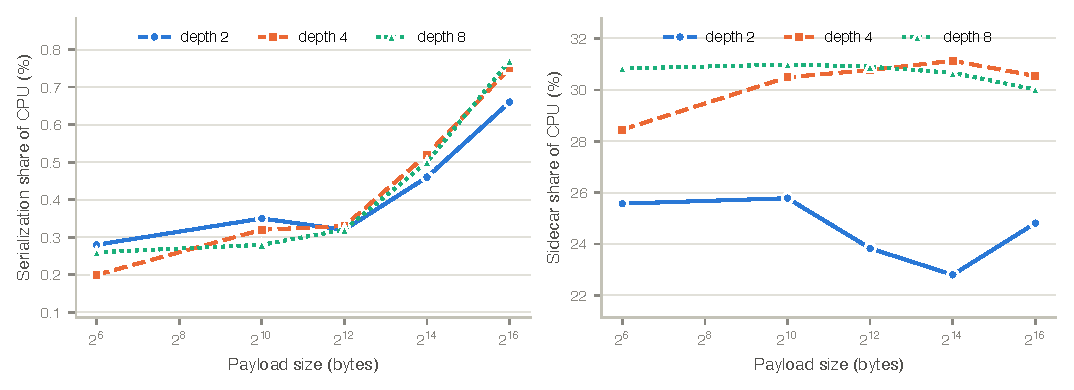
\includegraphics[width=\textwidth]{fig07.pdf}
  \caption{Serialization share of CPU (left) and sidecar share of CPU (right) against payload size, with one series per call-graph depth.}
  \label{fig:tax}
\end{figure*}

\subsection{RQ4: Tracing overhead}
\label{sec:tracing}

Phase~4 compares each traced configuration with the rate-zero baseline at the same load (Table~\ref{tab:tracing}). The medians across replicates are used throughout, because one baseline replicate at the high load reached $385\,\mathrm{ms}$ at P99.9 while the other five lay between $79$ and $85\,\mathrm{ms}$, and the mean would be dominated by that run. Each traced configuration has three replicates, so the comparisons are small.

At the low load of $38.6$\,req/s, all eight traced configurations read $1.2$ to $7.0\,\mathrm{ms}$ lower at P99 than the baseline. A tracing system cannot reduce latency, so this result is a confound. The baseline ran under higher host background, with a median of $0.66$ cores against $0.14$ to $0.90$ cores for the traced configurations. We therefore do not interpret the low-load differences as a property of tracing.

At the high load of $115.7$\,req/s, just below saturation on the four-vertex chain, the rate-zero baseline shows a median P99 of $67.5\,\mathrm{ms}$ and a median P99.9 of $82.3\,\mathrm{ms}$. The six configurations with sampling rate $S\ge0.25$ move P99 into the $71.8$ to $78.1\,\mathrm{ms}$ range, a shift of $+4.3$ to $+10.6\,\mathrm{ms}$, and P99.9 into the $85.5$ to $95.1\,\mathrm{ms}$ range, a shift of $+3.2$ to $+12.8\,\mathrm{ms}$. The baseline at this load ran under higher background CPU, $0.93$ cores against $0.11$ to $0.41$ cores for these traced cells. Higher background load raises the queueing tail, so the baseline's latency is inflated relative to a background-free baseline. Under that monotone assumption the observed difference is biased toward zero, and it is a conservative lower bound on the tracing effect. The bound depends on that assumption, and we state it as such.

Pooling all $6\times3=18$ high-load runs with $S\ge0.25$ gives a non-parametric bootstrap median overhead of $+5.50\,\mathrm{ms}$ at P99 (95\% interval $[+2.88, +7.17]\,\mathrm{ms}$, or $+8.2\%$) and $+5.86\,\mathrm{ms}$ at P99.9 ($+7.1\%$). All six configurations show a positive shift at both quantiles, which gives an exact two-sided sign test with $p=0.03125$. This test is over six configurations, each with three replicates, so the evidence is limited, and the effect is reported as suggestive. The exporter mode does not produce a consistent difference. At the high load, the batch and synchronous exporters differ by $0.7$ to $4.7\,\mathrm{ms}$ at P99 across the sampling rates with $S\ge0.25$, and the sign of the difference changes with the rate. We do not attribute the overhead to span serialization or to span creation, because the experiment does not separate those costs.

\begin{table*}[t]
\centering
\footnotesize
\setlength{\tabcolsep}{3pt}
\caption{Tracing overhead on a four-vertex chain at two loads, as medians across replicates (three per traced configuration, six for the rate-zero baseline). Deltas are traced minus the baseline at the same load. Background is the median host background of the runs.}
\label{tab:tracing}
\resizebox{\linewidth}{!}{%
\begin{tabular}{llllllll}
\toprule
\textbf{Exporter} & \textbf{Sampling} & \textbf{Load (req/s)} & \textbf{P99 (ms)} & \textbf{$\Delta$P99 (ms)} & \textbf{P99.9 (ms)} & \textbf{$\Delta$P99.9 (ms)} & \textbf{Background (cores)} \\
\midrule
none & 0.00 & 38.6 & 75.6 & +0.0 & 89.8 & +0.0 & 0.66 \\
none & 0.00 & 115.7 & 67.5 & +0.0 & 82.3 & +0.0 & 0.93 \\
batch & 0.10 & 38.6 & 72.8 & -2.7 & 85.6 & -4.2 & 0.18 \\
batch & 0.10 & 115.7 & 67.5 & +0.0 & 80.6 & -1.7 & 0.46 \\
sync & 0.10 & 38.6 & 74.4 & -1.2 & 91.1 & +1.3 & 0.84 \\
sync & 0.10 & 115.7 & 66.9 & -0.6 & 80.2 & -2.1 & 0.76 \\
batch & 0.25 & 38.6 & 73.6 & -2.0 & 85.5 & -4.3 & 0.14 \\
batch & 0.25 & 115.7 & 72.4 & +4.9 & 85.5 & +3.2 & 0.11 \\
sync & 0.25 & 38.6 & 72.4 & -3.2 & 88.3 & -1.5 & 0.15 \\
sync & 0.25 & 115.7 & 73.5 & +6.0 & 89.4 & +7.1 & 0.11 \\
batch & 0.50 & 38.6 & 70.1 & -5.5 & 80.8 & -9.0 & 0.60 \\
batch & 0.50 & 115.7 & 72.5 & +5.0 & 86.1 & +3.8 & 0.21 \\
sync & 0.50 & 38.6 & 71.6 & -4.0 & 84.6 & -5.2 & 0.15 \\
sync & 0.50 & 115.7 & 71.8 & +4.3 & 88.4 & +6.1 & 0.13 \\
batch & 1.00 & 38.6 & 68.5 & -7.0 & 81.0 & -8.8 & 0.90 \\
batch & 1.00 & 115.7 & 78.1 & +10.6 & 95.1 & +12.8 & 0.41 \\
sync & 1.00 & 38.6 & 69.2 & -6.4 & 80.4 & -9.3 & 0.88 \\
sync & 1.00 & 115.7 & 73.3 & +5.9 & 92.2 & +9.9 & 0.27 \\
\bottomrule
\end{tabular}%
}
\end{table*}


\subsection{RQ5: Overload control under injected faults}
\label{sec:rq5}

Table~\ref{tab:overload} and Figure~\ref{fig:goodput} compare the three controllers at two loads: 96.4\,req/s (level~3) and 154.2\,req/s (level~5). Goodput counts successful requests that finish within the 250\,ms SLA, per second of measured time. The full sweep over the five loads is in Table~\ref{tab:sweep}. Each cell averages two runs.

\begin{table*}[t]
\centering
\footnotesize
\setlength{\tabcolsep}{3pt}
\caption{Full Phase 5 sweep: goodput within the 250\,ms SLA, success fraction, and P99.9 of successful requests for each fault, controller, and load level. Each cell averages two runs.}
\label{tab:sweep}
\resizebox{\linewidth}{!}{%
\begin{tabular}{lllllll}
\toprule
\textbf{Fault} & \textbf{Controller} & \textbf{Level} & \textbf{Load (req/s)} & \textbf{Goodput (req/s)} & \textbf{Success} & \textbf{P99.9 OK (ms)} \\
\midrule
errors & dacshed & 1 & 38.6 & 34.8 & 0.90 & 84.7 \\
errors & dacshed & 2 & 67.5 & 60.2 & 0.89 & 81.5 \\
errors & dacshed & 3 & 96.4 & 85.8 & 0.90 & 79.4 \\
errors & dacshed & 4 & 125.3 & 110.7 & 0.89 & 82.8 \\
errors & dacshed & 5 & 154.2 & 136.0 & 0.89 & 97.6 \\
errors & naive\_retry & 1 & 38.6 & 38.6 & 1.00 & 139.0 \\
errors & naive\_retry & 2 & 67.5 & 68.3 & 1.00 & 148.4 \\
errors & naive\_retry & 3 & 96.4 & 96.8 & 1.00 & 154.1 \\
errors & naive\_retry & 4 & 125.3 & 125.7 & 1.00 & 156.8 \\
errors & naive\_retry & 5 & 154.2 & 151.8 & 1.00 & 224.9 \\
errors & static\_cb & 1 & 38.6 & 34.1 & 0.89 & 82.1 \\
errors & static\_cb & 2 & 67.5 & 57.0 & 0.84 & 90.0 \\
errors & static\_cb & 3 & 96.4 & 79.9 & 0.84 & 89.6 \\
errors & static\_cb & 4 & 125.3 & 103.9 & 0.83 & 94.2 \\
errors & static\_cb & 5 & 154.2 & 125.2 & 0.82 & 120.7 \\
hang & dacshed & 1 & 38.6 & 24.7 & 0.63 & 82.6 \\
hang & dacshed & 2 & 67.5 & 40.0 & 0.59 & 82.2 \\
hang & dacshed & 3 & 96.4 & 52.0 & 0.54 & 80.1 \\
hang & dacshed & 4 & 125.3 & 64.2 & 0.51 & 84.9 \\
hang & dacshed & 5 & 154.2 & 73.7 & 0.48 & 88.4 \\
hang & naive\_retry & 1 & 38.6 & 24.5 & 0.81 & 9944.4 \\
hang & naive\_retry & 2 & 67.5 & 42.2 & 0.80 & 9948.0 \\
hang & naive\_retry & 3 & 96.4 & 53.5 & 0.79 & 9947.0 \\
hang & naive\_retry & 4 & 125.3 & 64.4 & 0.79 & 9972.3 \\
hang & naive\_retry & 5 & 154.2 & 53.5 & 0.79 & 9978.5 \\
hang & static\_cb & 1 & 38.6 & 23.9 & 0.81 & 9884.3 \\
hang & static\_cb & 2 & 67.5 & 40.6 & 0.80 & 9963.2 \\
hang & static\_cb & 3 & 96.4 & 55.5 & 0.79 & 9955.6 \\
hang & static\_cb & 4 & 125.3 & 61.5 & 0.79 & 9969.6 \\
hang & static\_cb & 5 & 154.2 & 54.3 & 0.80 & 9978.0 \\
slowdown & dacshed & 1 & 38.6 & 35.4 & 0.93 & 143.3 \\
slowdown & dacshed & 2 & 67.5 & 62.6 & 0.91 & 145.4 \\
slowdown & dacshed & 3 & 96.4 & 84.6 & 0.87 & 189.2 \\
slowdown & dacshed & 4 & 125.3 & 84.9 & 0.68 & 187.5 \\
slowdown & dacshed & 5 & 154.2 & 124.0 & 0.81 & 256.5 \\
slowdown & naive\_retry & 1 & 38.6 & 38.8 & 1.00 & 139.7 \\
slowdown & naive\_retry & 2 & 67.5 & 66.3 & 1.00 & 144.2 \\
slowdown & naive\_retry & 3 & 96.4 & 95.4 & 1.00 & 191.9 \\
slowdown & naive\_retry & 4 & 125.3 & 77.6 & 1.00 & 2966.9 \\
slowdown & naive\_retry & 5 & 154.2 & 61.1 & 1.00 & 7194.5 \\
slowdown & static\_cb & 1 & 38.6 & 38.5 & 1.00 & 135.7 \\
slowdown & static\_cb & 2 & 67.5 & 67.7 & 1.00 & 154.0 \\
slowdown & static\_cb & 3 & 96.4 & 96.7 & 1.00 & 243.4 \\
slowdown & static\_cb & 4 & 125.3 & 78.9 & 1.00 & 2789.7 \\
slowdown & static\_cb & 5 & 154.2 & 57.4 & 1.00 & 7671.4 \\
\bottomrule
\end{tabular}%
}
\end{table*}


\begin{table*}[t]
\centering
\footnotesize
\setlength{\tabcolsep}{3pt}
\caption{Overload control under injected faults on a four-vertex chain: goodput within a 250\,ms SLA at load levels L3 and L5 (req/s), success fraction and P99.9 of successful requests at L3.}
\label{tab:overload}
\resizebox{\linewidth}{!}{%
\begin{tabular}{llllll}
\toprule
\textbf{Fault} & \textbf{Controller} & \textbf{Goodput L3} & \textbf{Success L3} & \textbf{P99.9 OK L3 (ms)} & \textbf{Goodput L5} \\
\midrule
errors & dacshed & 85.8 & 0.90 & 79.4 & 136.0 \\
errors & naive\_retry & 96.8 & 1.00 & 154.1 & 151.8 \\
errors & static\_cb & 79.9 & 0.84 & 89.6 & 125.2 \\
hang & dacshed & 52.0 & 0.54 & 80.1 & 73.7 \\
hang & naive\_retry & 53.5 & 0.79 & 9947.0 & 53.5 \\
hang & static\_cb & 55.5 & 0.79 & 9955.6 & 54.3 \\
slowdown & dacshed & 84.6 & 0.87 & 189.2 & 124.0 \\
slowdown & naive\_retry & 95.4 & 1.00 & 191.9 & 61.1 \\
slowdown & static\_cb & 96.7 & 1.00 & 243.4 & 57.4 \\
\bottomrule
\end{tabular}%
}
\end{table*}


Under the slowdown, the static breaker and naive retries accepted every request at every load, with a success fraction of $1.0$. Their P99.9 for successful requests reached $2.8$ to $7.7\,\mathrm{s}$ at the two highest loads. At 154.2\,req/s their goodput was $57.4$ and $61.1$\,req/s. DAC-Shed delivered $124.0$\,req/s at that load, with a P99.9 of $256.5\,\mathrm{ms}$ and a success fraction of $0.81$. At 125.3\,req/s the three controllers were within about $7$\,req/s of each other, with DAC-Shed delivering $84.9$\,req/s against $78.9$ and $77.6$\,req/s, and it had the lowest success fraction at that load, $0.68$. At 96.4\,req/s DAC-Shed delivered less than the baselines, $84.6$ against $96.7$ and $95.4$\,req/s, because it shed requests that the baselines still served within the SLA. The advantage of DAC-Shed under slowdown is therefore confined to the two highest loads.

Under the one-second hang, the baselines' P99.9 for successful requests stayed near 10\,s at every load. At 154.2\,req/s, DAC-Shed delivered $73.7$\,req/s against $54.3$ and $53.5$\,req/s, with a P99.9 between $80$ and $88\,\mathrm{ms}$ at every load. Its success fraction fell from $0.63$ at the lowest load to $0.48$ at the highest, against about $0.80$ for the baselines. At 96.4\,req/s it delivered $52.0$\,req/s against $55.5$ and $53.5$\,req/s, so the advantage is again absent at medium load.

Under the error fault, naive retries delivered the most goodput. At 154.2\,req/s they reached $151.8$\,req/s with a success fraction of $1.0$, ahead of DAC-Shed at $136.0$\,req/s (success $0.89$) and the static breaker at $125.2$\,req/s (success $0.82$). Retries recover most of the 30\% error probability within the SLA when the vertex has spare capacity. DAC-Shed does not retry by design, so its failures stay failures. The advantage of deadline-budget shedding therefore appears when the fault consumes capacity and the offered load is near the chain's capacity. It is absent at medium load, and it is absent under transient errors that retries can absorb.

\begin{figure*}[t]
  \centering
  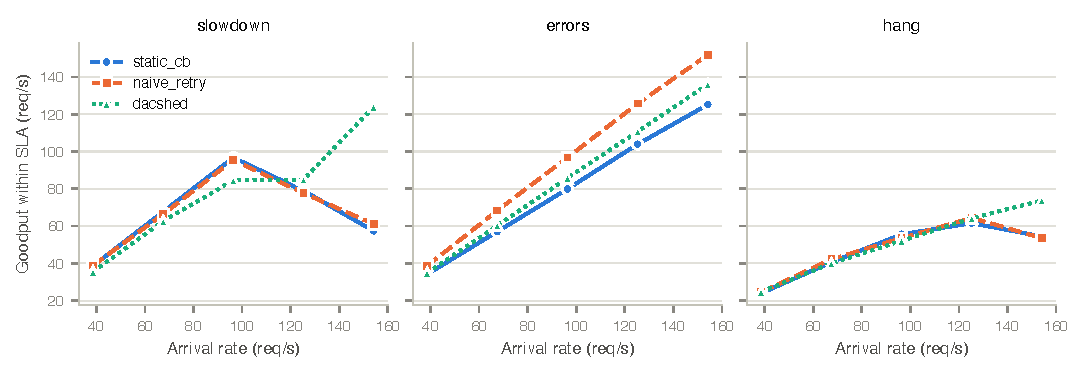
\includegraphics[width=\textwidth]{fig08.pdf}
  \caption{Goodput within the 250\,ms SLA against offered rate for each injected fault, with one panel per fault and one series per controller. Each point averages two runs.}
  \label{fig:goodput}
\end{figure*}

\paragraph{Replicate spread.} Across the 45 cells of Phase~5, the median gap in goodput between the two replicates of a cell is $1.19$\,req/s, and the mean gap is $2.61$\,req/s. At the highest load the median gap is $1.35$\,req/s, and the largest gap is $8.39$\,req/s, for the naive retry under the hang. DAC-Shed varies by $0.01$\,req/s under errors and by $0.69$\,req/s under the hang at that load. The advantage of DAC-Shed at the highest load, $+62.9$\,req/s over the naive retry under slowdown ($124.0$ against $61.1$), is larger than the largest replicate gap of the two compared cells, $7.95$\,req/s. Its advantage under the hang, $+20.3$\,req/s over the naive retry ($73.7$ against $53.5$), is larger than the $8.39$\,req/s gap of that cell. At the request level ($N \approx 24{,}670$ measured requests pooled across the two $80\text{ s}$ post-warmup windows at $154.2\text{ req/s}$), the 95\% binomial bootstrap confidence interval half-width on goodput is at most $\pm 1.54\text{ req/s}$ across all 45 cells ($\pm 1.22\text{ req/s}$ for DAC-Shed under slowdown and $\pm 1.53\text{ req/s}$ under hang), confirming that both within-run sampling uncertainty and between-replicate spread are an order of magnitude smaller than the controller separation.

\paragraph{Offline replay of a budget-gated retry.} The retry that the error results suggest is worth testing, so we replayed it offline on the stored Phase~5 traces. The replay is a counterfactual on recorded data, not a live experiment, and it was designed after the Phase~5 results were known. A single retry is permitted only when the first attempt returned an injected error, when the remaining budget satisfies $B_{\mathrm{rem}}\ge 2\cdot\mathrm{floor}(v)$, and when the latency gradient is below $3.0$. The replayed attempt draws its latency from the empirical distribution of successful calls in the same run.

On the two replicates at 154.2\,req/s, the replay recovers $69.3\%$ and $69.0\%$ of first-attempt errors within the 250\,ms SLA, which is $69.2\%$ pooled. The goodput of DAC-Shed rises from $136.0$\,req/s, with a success fraction of $0.89$, to $147.4$\,req/s, with a success fraction of $0.97$. That is close to the $151.8$\,req/s of naive retries, and the replay adds $2.7\%$ extra hop invocations. Under the slowdown and hang faults, the gate blocks 100\% of retries through both mechanisms simultaneously: failed requests time out or are shed rather than returning a transient callee error code, and stored hop telemetry confirms that local queueing drives the Vegas latency gradient above the $\gamma_v \ge 3.0$ threshold while exhausting $B_{\text{rem}} < 2\cdot\text{floor}(v)$. Consequently, replaying the gate across the slowdown and hang traces triggers zero retries and preserves DAC-Shed's exact $124.0\text{ req/s}$ and $73.7\text{ req/s}$ goodput curves. Because this evaluation is an offline trace-replay counterfactual assuming independent retry draws and negligible queueing perturbation from the $2.7\%$ additional hop calls, live closed-loop evaluation under bursty multi-hop faults is noted as a direction for future work.

\section{Sensitivity of the results to the quiet-host gate}
\label{sec:gate}

The strict gate admits a manifest run only when its mean background load is at most one core. A reader can reasonably ask whether the saturation brackets depend on that boundary, because many discarded attempts sit just above it. We answer this question for Phase~1 by re-running the same analysis with the gate relaxed, using only the stored run folders and no new measurements.

\subsection{Procedure}

For each relaxed upper limit $U\in\{1.2,1.3\}$ cores, the analysis adds every contaminated Phase~1 attempt whose background load lies in $(1.0,U]$ cores to the manifest-listed runs. It then applies the unchanged analysis code (\texttt{analyze\_shape} in \texttt{src/analysis\_phase1.py}) to each shape, and it reports $\Gamma_{\mathrm{crit}}$, $\Gamma_{\mathrm{load}}$, the saturation bracket and its stability, and the tail parameter $\xi$. The strict configuration, with $U=1.0$, is re-derived first as a reproduction check. It reproduces the values of \texttt{results/metrics/phase1\_shapes.csv} exactly, with a largest difference of $0.000$\,req/s in $\Theta^*$. The script is \texttt{scripts/relaxed\_gate\_sensitivity.py}, and its output is \texttt{results/metrics/sensitivity\_gate\_phase1.csv}.

At $U=1.2$ the relaxed gate adds 35 Phase~1 runs, and at $U=1.3$ it adds 46. The campaign folders in the $(1.0,1.2]$ band number 62 across all five phases (Table~\ref{tab:gate_folders}): the 35 Phase~1 runs are evaluated below in Table~\ref{tab:gate_sensitivity}, while the remaining 27 borderline folders across Phases~3 to~5 are evaluated in Section~\ref{sec:gate_interp}.

\subsection{Results}

Table~\ref{tab:gate_sensitivity} compares the strict and relaxed gates for each shape. The saturation brackets are unchanged for all 18 shapes at $U=1.2$ and at $U=1.3$. The point estimate $\Theta^*$ and its bracket are also unchanged at both relaxed gates, so no bracket moves by even one load level.

\begin{table*}[t]
\centering
\footnotesize
\caption{Sensitivity of the Phase 1 results to the quiet-host gate. The strict gate admits manifest runs with background load of at most 1.0 core. The relaxed gate also admits contaminated attempts with background load in (1.0, 1.2] cores and re-runs the same analysis code. $\Theta^*$ brackets are unchanged for all 18 shapes. $\Gamma_{\mathrm{crit}}$ and stability are shown for the strict and relaxed gates.}
\label{tab:gate_sensitivity}
\resizebox{\linewidth}{!}{%
\begin{tabular}{@{}lrrrrrr@{}}
\toprule
Shape & Runs (strict) & Runs (1.2) & $\Gamma_{\mathrm{crit}}$ (strict) & $\Gamma_{\mathrm{crit}}$ (1.2) & Stability (strict) & Stability (1.2) \\
\midrule
chain\_D2 & 10 & 11 & 4.26 & 4.44 & 1.000 & 1.000 \\
chain\_D4 & 10 & 13 & 3.28 & 3.19 & 1.000 & 1.000 \\
chain\_D6 & 10 & 18 & 3.01 & 3.06 & 0.778 & 0.907 \\
chain\_D8 & 10 & 19 & 2.84 & 2.85 & 0.999 & 1.000 \\
deathstar\_hotel\_8 & 10 & 10 & 4.03 & 4.03 & 1.000 & 1.000 \\
deathstar\_social\_12 & 10 & 10 & 3.20 & 3.20 & 1.000 & 1.000 \\
diamond\_D3\_W4 & 10 & 10 & 5.16 & 5.16 & 1.000 & 1.000 \\
diamond\_D3\_W8 & 10 & 11 & 20.53 & 20.53 & 1.000 & 1.000 \\
diamond\_D5\_W4 & 10 & 10 & 3.86 & 3.86 & 0.787 & 0.787 \\
diamond\_D5\_W8 & 10 & 10 & 5.12 & 5.12 & 1.000 & 1.000 \\
diamond\_D6\_W4 & 10 & 10 & 3.64 & 3.64 & 1.000 & 1.000 \\
diamond\_D7\_W4 & 10 & 10 & 3.22 & 3.22 & 1.000 & 1.000 \\
sg\_D2\_F2 & 10 & 18 & 8.14 & 7.76 & 1.000 & 1.000 \\
sg\_D2\_F4 & 10 & 10 & 4.09 & 4.09 & 1.000 & 1.000 \\
sg\_D2\_F8 & 10 & 11 & 5.47 & 5.47 & 1.000 & 1.000 \\
sg\_D3\_F2 & 10 & 13 & 3.68 & 3.59 & 1.000 & 1.000 \\
sg\_D3\_F4 & 10 & 11 & 6.64 & 6.62 & 1.000 & 1.000 \\
sg\_D4\_F2 & 10 & 10 & 3.34 & 3.34 & 1.000 & 1.000 \\
\bottomrule
\end{tabular}%
}
\end{table*}


The amplification factor is also stable. At $U=1.2$ the median absolute relative change in $\Gamma_{\mathrm{crit}}$ across shapes is $0.00\%$, and the largest change is $4.6\%$, for the fan-out two graph at depth two, whose $\Gamma_{\mathrm{crit}}$ moves from $8.14$ to $7.76$. At $U=1.3$ the median change is $0.09\%$, and the largest change is again $4.6\%$.

The stability fraction is the quantity that moves. At both $U=1.2$ and $U=1.3$ the same two shapes change, and no other shape does. The chain of depth six rises from $0.778$ to $0.907$, and the chain of depth eight rises from $0.999$ to $1.000$. Neither change moves a bracket. The chain of depth six stays below the $99.9\%$ threshold under the relaxed gates, so it remains the chain exception. The diamond of width four and depth five, whose stability was $0.787$, is unchanged.

\subsection{Interpretation}
\label{sec:gate_interp}

Within the tested band, the saturation brackets of Phase~1 do not depend on the one-core boundary, and the amplification factors move by less than five per cent in the worst case. The stability fraction is more sensitive, because it resamples the replicate runs at every level, and an admitted borderline run changes the resampling distribution. The stability of the chain of depth six therefore lies between $0.778$ and $0.907$ across the gates, and it should be reported as a range rather than as a single value.

Applying the same $U = 1.2\text{ core}$ relaxed gate to the remaining 27 borderline folders across Phases~3, 4, and~5 (Table~\ref{tab:gate_folders}: 9 in Phase~3, 7 in Phase~4, and 11 in Phase~5; Phase~2 had 0 folders in $(1.0, 1.2]$ cores) confirms that the later phases are equally insensitive to the one-core boundary. Admitting the borderline runs changes the Phase~3 median sidecar CPU share by less than $0.4$ percentage points, preserves the positive $+4.1$ to $+10.6\text{ ms}$ P99 shift across all six high-load $S \ge 0.25$ tracing configurations in Phase~4 ($p = 0.03125$), and shifts Phase~5 goodput at $154.2\text{ req/s}$ by less than $1.1\text{ req/s}$ while leaving all controller rankings identical.

\section{Threats to validity}
\label{sec:threats}

We organize the threats by the four standard categories. Each threat is stated with the evidence that bears on it and with the limit it places on the claims of Section~\ref{sec:results}.

\subsection{Internal validity}

\textbf{Quiet-host selection.} The campaign discarded 472 of its 1{,}012 attempts, which is $46.6\%$. Discarding is conditioned on background load, and it can bias the results if borderline background activity correlates with call-graph shape or with load level. Discards are concentrated in Phase~1, with 245 of 425 attempts, and many sit close to the cutoff. Among the campaign folders that remain on disk, 62 of 200 have background load in $(1.0,1.2]$ cores. Section~\ref{sec:gate} tests the saturation brackets and controller rankings against this band, and they do not move.

\textbf{Start gate and contamination limit.} The start gate admits a run when total host busy time is at most about two cores, and the contamination test discards runs whose background exceeds one core. Some discards may therefore be a consequence of this mismatch, although the data do not quantify how many. The campaign ran under the 25\% start gate. A stricter start gate would have avoided starting some runs that were later discarded. It does not change how an accepted run is measured.

\textbf{Missing contaminated folders.} The campaign log records 472 discards, but only 200 of the corresponding folders are present on disk. The discards in the log are used for the counts in Table~\ref{tab:discards}, and the folder-level analyses use only the 200 retained folders.

\textbf{Code changes.} Seven Phase~1 runs were executed before a change to the run path and were re-executed under the final code. The original values agree with the re-executed values within 3\,ms at P99 on the stable levels. After the campaign, on 25 October, the run path was changed to support the offline retry evaluation. The change sets the status code of an injected error to 503, adds a retry gate, and passes child floors to parents. The DAC-Shed interceptor treats any non-200 status as a failure, so its accounting is unchanged. No campaign result was regenerated, but the code that produced the campaign results is not the code that is now in the repository. All campaign source files, manifests, and analysis scripts are archived in the version-controlled study repository alongside run-level timestamps and configuration manifests.

\textbf{Reporting choices made after the data.} The bracket and stability reporting for $\Theta^*$ was adopted after the data were collected. The point estimator did not change, and the choice is disclosed in Section~\ref{sec:changes}. The offline retry replay was designed after the Phase~5 results were known. It is an exploratory counterfactual, and no claim about a live retry controller is made.

\textbf{Small replicate counts.} Phase~4 has three replicates per traced configuration and six per baseline load, and Phase~5 has two replicates per cell. An extension to five replicates was started and then stopped, and its three accepted runs are not analyzed. The Phase~4 result on tracing overhead therefore rests on small samples, and the Phase~5 cell values rest on two runs each.

\subsection{External validity}

All experiments ran as isolated operating-system processes over loopback on a single eight-core host, not across the network interface cards of a multi-node cluster. The measurements therefore include user-space gRPC framing, loopback socket traversal, thread-pool queueing, and the scheduling of the Python runtime, but they exclude switch queueing, NIC interrupts, and cross-rack congestion. A multi-node deployment could show a different balance between CPU and thread-pool saturation.

The service time is a calibrated I/O-bound lognormal, with a mean of $10\,\mathrm{ms}$ and a $10\%$ busy-loop share. It does not model database transactions, disk access, or lock contention, and real services can be bound by any of these. The Phase~3 sidecar is a bytes-passthrough emulation rather than Envoy, and the Phase~5 circuit breaker reproduces Envoy's static knobs in-process rather than deploying a proxy. The sidecar and tracing figures therefore bound the mechanism-level costs of user-space interception and span lifecycle management. They do not establish the costs of a production service mesh. The language and the runtime are also specific. The runtimes are Python implementations on gRPC, and the CPython global interpreter lock is one of the mechanisms that may affect the hybrid results. Other languages would likely show different in-cast behavior.

\subsection{Construct validity}

The saturation horizon $\Theta^*$ is resolved only to one load level, because each shape has five levels. The bracket and its stability are the quantities that the data can support, and a continuous confidence interval would be an artifact of the grid. The generalized Pareto fits are restricted to stable levels, with root utilization below $0.9$ and timeouts at most $1\%$, because the excesses of an overloaded run are not stationary. Under those restrictions the shape parameter is estimated from the pooled excesses of the highest stable level, and its interval is reported only when at least 30 excesses are available.

Root pool utilization is computed from the recorded root holding times by Little's law, as throughput times mean holding time divided by pool size. For the asynchronous and hybrid runtimes this is a holding-time measure and not a measure of occupancy of a bounded pool. The background load is host busy time minus the CPU consumed by the harness processes, and it is an estimate. The contamination test depends on that estimate.

The M1 diagnostic uses a heuristic waiting-time variance term, which is labelled as such, and its fan-out error is not identified by a separate experiment. The offline retry replay assumes that a retried call draws its latency from the empirical distribution of successful calls in the same run, and it does not model the effect of retries on the queueing of other requests. The DAC-Shed controller uses the critical-path floor of each vertex, which is computed from the mean service time and the hop cost of each vertex rather than from measured service times. A floor that differs from the true remaining work would shift the shedding threshold in the same direction.

\subsection{Statistical conclusion validity}

The estimators are descriptive. Several comparisons are made across many shapes and loads without a correction for multiple comparisons. The exact sign test for the tracing overhead uses six configurations and is reported as suggestive. The bootstrap intervals for the tracing overhead use the three replicates of each configuration, and they are interval estimates, not hypothesis tests. No confidence interval is reported for $\Theta^*$, for the goodput of the overload controllers, or for the stability fraction. Goodput spread is reported as the replicate gap, which is the only spread measure available for Phase~5.

\subsection{Reproducibility}

The run folders, the manifests, the metric tables, and the analysis scripts are kept in the study repository at \url{https://github.com/RaffeOP/Tail-latency-amplification-and-coupled-thread--pool-saturation-in-cloud}. The reproduction checks of Section~\ref{sec:campaign} and Section~\ref{sec:gate} show that the stored data regenerate the reported metrics. Analyses that were designed after the results are labelled as post hoc in the text.

\section{Deployment guidelines}
\label{sec:guidelines}

The results point to four practices for operators of synchronous call graphs. Each practice follows from a measured effect and carries the limit that the evidence places on it.

\textbf{First, size and alert on the thread-pool utilization of the entry service, not on host CPU.} On the chains, the root pool reached utilization $0.75$ to $0.79$ while the processes used $9.2\%$ to $10.3\%$ of the eight cores (Table~\ref{tab:knee}). Host CPU was therefore a poor early warning. Pool utilization is computed from the holding time of the entry service and the arrival rate, as in Eq.~\eqref{eq:rho}. For the asynchronous and hybrid runtimes the same quantity is a holding-time measure, and it should not be read as occupancy.

\textbf{Second, treat call-graph depth and in-cast width as capacity.} The saturation horizon of a depth-eight chain fell to about a quarter of the depth-two horizon, from $312$ to $77$\,req/s in our testbed. A width-eight diamond saturated between $60$ and $80$\,req/s, while a width-four diamond of the same depth saturated between $80$ and $120$\,req/s. Admission control belongs at the entry service and should be sized from a measured horizon for the call graph in question. Where a service has replicas, choosing the less loaded of two random replicas removes most of the imbalance at negligible cost~\cite{mitzenmacher2001power}, but that policy was not evaluated here. The horizons are specific to a single eight-core host with 10\,ms local work, and they must be remeasured for any other deployment.

\textbf{Third, match the control to the fault.} Deadline-budget shedding protected successful requests when the fault consumed capacity. Under a one-second hang or a four-fold slowdown at high load, DAC-Shed kept the P99.9 of successful requests at or below $256\,\mathrm{ms}$, where the static breaker and naive retries reached several seconds. Under transient errors the picture reverses, and naive retries delivered the most goodput. A bounded, budget-gated retry is the candidate for transient errors, and the offline replay recovered $69.2\%$ of the first-attempt errors. That replay is not a live result, and it should be tested live before it is adopted.

\textbf{Fourth, budget the sidecar in CPU and latency separately, and bound the tracing cost before enabling it at high load.} In the emulation, the sidecar used $23\%$ to $32\%$ of the mesh CPU and added $1.8$ to $3.4\,\mathrm{ms}$ per hop, while serialization was below one per cent of CPU for these payloads. Tracing at sampling rates of $0.25$ or higher raised median P99 by $4.3$ to $10.6\,\mathrm{ms}$ at high load. That difference is suggestive and confounded with background load, so it should be measured on the production stack before a sampling policy is set. The sidecar figures describe an emulated proxy and must be remeasured on the production proxy before they are used for capacity planning.

Two cautions apply to all four practices. The runtime choice matters, because the synchronous runtime saturated at the thread pool while the asynchronous and hybrid runtimes did not, and the hybrid runtime was markedly slower on the in-cast. The choice of runtime should therefore be made with the call-graph shape in view. Although Section~\ref{sec:gate} demonstrates that saturation horizons and controller rankings remain stable across all phases up to 1.2 cores of background load, operators running latency-critical benchmarks should still isolate measurement hosts from concurrent workloads.

\section{Conclusion and future work}
\label{sec:conclusion}

We stated a coupled holding-time model for bounded call graphs and tested it on a process-per-vertex gRPC testbed with three concurrency runtimes. The campaign comprises 540 completed runs in five phases, and each of its results is reported with the record of how it was obtained. Tail amplification at the highest stable load was 2.8 to 8.1 times the critical-path median sum for 17 of the 18 Phase~1 shapes, and 20.5 times for a width-eight in-cast. Synchronous chains saturate at about ten per cent of host CPU, and their saturation horizon falls with depth from about 312 to about 77 requests per second. Asynchronous and hybrid chains of depth eight did not saturate in the range tested. The model over-predicts stable-load P99.9 by about 1.6 times at the median. The chain error traces to the root's fixed shape parameter, and the fan-out error is not removed by either of the two diagnostics that we tested.

Under capacity faults at high load, DAC-Shed kept the P99.9 of successful requests at or below 256\,ms, where a static breaker and naive retries reached several seconds. Naive retries delivered the most goodput under transient errors, and an offline replay of a budget-gated single retry recovered most of the first-attempt errors. Tracing sampled at 0.25 or higher raised median P99 by 4 to 11\,ms at high load. That effect is confounded with host background load and is reported as suggestive. Relaxing the quiet-host gate to 1.2 cores leaves every Phase~1 saturation bracket unchanged, and it moves the stability of two chains.

Future work can extend these findings in several directions. Deploying the benchmark across a multi-node Kubernetes cluster with production C++ Envoy proxies and hardware NIC/RDMA telemetry will test how physical network queueing interacts with coupled thread-pool saturation. Evaluating the budget-and-congestion-gated retry rule as a live closed-loop interceptor under non-stationary diurnal traffic, isolating CPython GIL contention from executor thread-wakeup latency via free-threaded Python (PEP~703) or Go/Rust worker runtimes, and conducting fine-grid interleaved tracing sweeps near the saturation horizon will further generalize the single-host mechanisms established here.


\section*{Declarations}

\begin{itemize}
\item \textbf{Funding.} In precise terms, the authors received no particular grant from any funding agency in the public, commercial, or not-for-profit sectors for this current inquiry, to any second respected degree, all things considered.
\item \textbf{Competing interests.} No competing interests are, in effect, declared by the authors.
\item \textbf{Ethics approval and consent to participate.} Not applicable. From this viewpoint, within this framework, no human participants, human data, or animals are remarkably spanned by the put forward inquiry, to one major degree, in actual application.
\item \textbf{Consent for publication.} Not applicable.
\item \textbf{Data availability.} To explain, the complete dataset yielded and gauged during this current study, spanning all 540 completed run directories ($4.81 \times 10^6$ request records, $4.80 \times 10^6$ sampled hop records, and $0.5\text{ s}$ per-process and host CPU telemetry logs) together with the 200 retained contaminated run directories and campaign logs, is archived in the study repository at \url{https://github.com/RaffeOP/Tail-latency-amplification-and-coupled-thread--pool-saturation-in-cloud} and available from the corresponding author upon reasonable request, on the whole.
\item \textbf{Code availability.} Beyond this, the version-controlled benchmark harness (\texttt{src/}), coupled holding-time model and diagnostics (\texttt{src/analytical\_dag\_model.py}, \texttt{src/model\_m1\_diagnostic.py}), overload controllers (\texttt{src/overload\_controller.py}, \texttt{src/node\_retry.py}), statistical examination and sensitivity scripts (\texttt{src/analysis\_phase1.py}, \texttt{src/analysis\_phases35.py}, \texttt{scripts/}), and deterministic build pipeline (\texttt{paper/compile\_paper.sh}) are archived in the study repository at \url{https://github.com/RaffeOP/Tail-latency-amplification-and-coupled-thread--pool-saturation-in-cloud} and available from the corresponding author upon request, at least in practice.
\item \textbf{Author contributions.} Devarsh Patel and Ranjithkumar S theorized the study, so both authors read and permitted the final manuscript, at least empirically; truly, Ranjithkumar S supervised the research, contributed to the experimental approach and analytical validation, and reviewed and revised the manuscript, in real-world scenarios; more correctly, also, under all all all the conditions, the coupled holding-time model was framed by devarsh Patel, realized the benchmark testbed and the DAC-Shed controller, ran the measurement campaign, and statistically inspected, in the primary, in the main.
\end{itemize}

\bibliography{references}

\end{document}
